\documentclass[10pt,journal,compsoc]{IEEEtran}

\usepackage{lineno,hyperref}
\modulolinenumbers[5]


% *** CITATION PACKAGES ***
%
\ifCLASSOPTIONcompsoc
  % IEEE Computer Society needs nocompress option
  % requires cite.sty v4.0 or later (November 2003)
  \usepackage[nocompress]{cite}
\else
  % normal IEEE
  \usepackage{cite}
\fi




\usepackage[font=footnotesize]{subfig, caption}
\usepackage{graphicx}
  \graphicspath{{./img/}}
  \DeclareGraphicsExtensions{.pdf,.jpeg,.png,.jpg}

\usepackage{todonotes}
\newcommand{\tododl}[1]{\todo[backgroundcolor=pink,size=\tiny]{DL: #1}}
\newcommand{\todoindl}[1]{\todo[inline,backgroundcolor=pink]{DL: #1}}
\newcommand{\todocdf}[1]{\todo[backgroundcolor=blue!20,size=\tiny]{CDF: #1}}
\newcommand{\todofc}[1]{\todo[backgroundcolor=yellow,size=\tiny]{FC: #1}}


\usepackage{xcolor}
\newcommand{\tcolor}[2]{\color{#1}{#2}\color{black}}
\usepackage{tabularx}
\usepackage{makecell}

\usepackage{amsmath}

\usepackage{outlines}
\usepackage[nolist]{acronym}
\usepackage{amssymb}

\usepackage{algorithm}%,algorithmic}

\usepackage{algpseudocode}
\algdef{SE}[SUBALG]{Indent}{EndIndent}{}{\algorithmicend\ }%
\algtext*{Indent}
\algtext*{EndIndent}

\usepackage{colortbl}



% \makeatletter
% \algrenewcommand\ALG@beginalgorithmic{\footnotesize}
% \makeatother



\usepackage{amsthm}

\theoremstyle{definition}
\newtheorem{definition}{Definition}[section]
\newtheorem{theorem}{Theorem}[section]
\newtheorem{lemma}{Lemma}[section]
\newtheorem{remark}{Remark}[section]

\theoremstyle{plain}
\newtheorem{example}{Example}[section]



\usepackage[inline]{enumitem}

\usepackage{xfp}

\usepackage{booktabs}
\usepackage{multirow}
%\usepackage{lmodern}
\usepackage[T1]{fontenc}


\usepackage{xspace}

%%%%%%%%%%%%%%%% MODIFY HERE FOR BLUE CHANGES
\newcommand{\blue}{blue}

\usepackage{listings}
\lstdefinestyle{base}{
moredelim=**[is][\color{\blue}]{�}{�},
}

\newcommand{\nd}{\texttt{NegDis}\xspace}
\newcommand{\declare}{\texttt{Declare}\xspace}
\newcommand{\rum}{\texttt{RuM}\xspace}
\newcommand{\declareminer}{\texttt{DeclareMiner}\xspace}
\newcommand{\decminer}{\texttt{DecMiner}\xspace}
\newcommand{\minclos}{\textsc{Cardinality}\xspace}
\newcommand{\subsetclos}{\textsc{Subset}\xspace}
\newcommand\dec[1]{$\mathsf{#1}$}
\newcommand\para[1]{\textnormal{\textsf{#1}}}

%%%%%%%%%%%%%%%% MODIFY HERE FOR BLUE CHANGES
\newcommand\btext[1]{{\tcolor{\blue}{#1}}}
\newcommand\paragrafo[1]{{\smallskip \noindent \textit{#1}.}}

\newcommand{\ltl}{LTL\xspace}
\newcommand{\ltlf}{LTL\ensuremath{_f}\xspace}




% MarcoM non condivide il termine choices, dice che è misunderstanding
% A tal scopo ho quindi creato una macro per deicedere che nome usare
% le sue proposte sono: negative witneses, discarders, rejecters, sheriffs marshals
\newcommand{\sheriff}{sheriffs}


%%%%%%%%%%%%%%%%%%%%%%%
%% Elsevier bibliography styles
%%%%%%%%%%%%%%%%%%%%%%%
%% To change the style, put a % in front of the second line of the current style and
%% remove the % from the second line of the style you would like to use.
%%%%%%%%%%%%%%%%%%%%%%%

%% Numbered
%\bibliographystyle{model1-num-names}

%% Numbered without titles
%\bibliographystyle{model1a-num-names}

%% Harvard
%\bibliographystyle{model2-names.bst}\biboptions{authoryear}

%% Vancouver numbered
%\usepackage{numcompress}\bibliographystyle{model3-num-names}

%% Vancouver name/year
%\usepackage{numcompress}\bibliographystyle{model4-names}\biboptions{authoryear}

%% APA style
%\bibliographystyle{model5-names}\biboptions{authoryear}

%% AMA style
%\usepackage{numcompress}\bibliographystyle{model6-num-names}

%% `Elsevier LaTeX' style
%\bibliographystyle{elsarticle-num}

%%%%%%%%%%%%%%%%%%%%%%%%%%%%%%%%%%%%%%%%%%%%%%%%%%%%%%%%%%%%%%%%%%%%%%%%%%%%%%%%%%%%%%%%%%%%

\begin{document}


\title{Process discovery on deviant traces\\ and other stranger things}

\author{Federico~Chesani, Chiara~Di~Francescomarino, Chiara~Ghidini, Daniela~Loreti, Fabrizio~Maria~Maggi, Paola~Mello, Marco~Montali, Sergio~Tessaris% <-this % stops a space
\IEEEcompsocitemizethanks{\IEEEcompsocthanksitem F.~Chesani, D.~Loreti, and P.~Mello are with DISI - University of Bologna, Italy. 
E-mail: daniela.loreti@unibo.it
\IEEEcompsocthanksitem C.~Di~Francescomarino and C.~Ghidini with Fondazione Bruno Kessler, Italy.
\IEEEcompsocthanksitem F.~M.~Maggi, M.~Montali, and S.~Tessaris are with Free University of Bozen/Bolzano, Italy.
}% <-this % stops an unwanted space
\thanks{Manuscript received April 19, 2005; revised August 26, 2015.}}


% The paper headers
\markboth{Journal of \LaTeX\ Class Files,~Vol.~14, No.~8, August~2015}%
{Shell \MakeLowercase{\textit{et al.}}: Bare Demo of IEEEtran.cls for Computer Society Journals}


\IEEEtitleabstractindextext{%
\begin{abstract}
As the need to understand and formalise business processes into a model has grown over the last years, 
the process discovery research field has gained more and more importance, developing two different classes of approaches to model representation: procedural and declarative. 
%
Orthogonally to this classification, the vast majority of works envisage the discovery task as a one-class supervised learning process guided by the traces that are recorded into an input log. 

In this work instead, we focus on declarative processes and embrace the less-popular view of process discovery as a binary supervised learning task, where the input log reports both examples of the normal system execution, and traces representing \btext{a ``stranger'' behaviour } according to the domain semantics. We therefore deepen how the valuable information brought by both these two sets can be extracted and formalised into a model that is ``optimal'' according to user-defined goals. Our approach, namely \nd, is evaluated w.r.t. other relevant works in this field, and shows promising results \btext{regarding } both the performance and the quality of the obtained solution.
\end{abstract}

% Note that keywords are not normally used for peerreview papers.
\begin{IEEEkeywords}
Process discovery, declarative process models, binary classification task.
\end{IEEEkeywords}}


% make the title area
\maketitle


% To allow for easy dual compilation without having to reenter the
% abstract/keywords data, the \IEEEtitleabstractindextext text will
% not be used in maketitle, but will appear (i.e., to be "transported")
% here as \IEEEdisplaynontitleabstractindextext when the compsoc 
% or transmag modes are not selected <OR> if conference mode is selected 
% - because all conference papers position the abstract like regular
% papers do.
\IEEEdisplaynontitleabstractindextext
% \IEEEdisplaynontitleabstractindextext has no effect when using
% compsoc or transmag under a non-conference mode.



% For peer review papers, you can put extra information on the cover
% page as needed:
% \ifCLASSOPTIONpeerreview
% \begin{center} \bfseries EDICS Category: 3-BBND \end{center}
% \fi
%
% For peerreview papers, this IEEEtran command inserts a page break and
% creates the second title. It will be ignored for other modes.
\IEEEpeerreviewmaketitle



% \IEEEraisesectionheading{\section{Introduction}\label{sec:introduction}}
% % Computer Society journal (but not conference!) papers do something unusual
% % with the very first section heading (almost always called "Introduction").
% % They place it ABOVE the main text! IEEEtran.cls does not automatically do
% % this for you, but you can achieve this effect with the provided
% % \IEEEraisesectionheading{} command. Note the need to keep any \label that
% % is to refer to the section immediately after \section in the above as
% % \IEEEraisesectionheading puts \section within a raised box.
%
% \IEEEPARstart{T}{his} demo file is intended to serve as a ``starter file''
% for IEEE Computer Society journal papers produced under \LaTeX\ using
% IEEEtran.cls version 1.8b and later.
% % You must have at least 2 lines in the paragraph with the drop letter
% % (should never be an issue)
% I wish you the best of success.
%
% \hfill mds
%
% \hfill August 26, 2015
%
%



%\linenumbers

% !TEX root = ../deviant-tkde.tex

\IEEEraisesectionheading{\section{Introduction}\label{sec:intro}}
\IEEEPARstart{T}{he} modelling of business processes is an important task to support decision-making in complex industrial and corporate domains. Recent years have seen the birth of the \ac{BPM} research area, focused on the analysis and control of process execution quality, and in particular, the rise in popularity of \emph{process mining} \cite{2012-Aalst}, which encompasses a set of techniques to extract valuable information from event logs. 
%
\emph{Process discovery} is one of the most investigated process mining techniques. It deals with the automatic learning of a process model from a given set of logged traces, each one representing the digital footprint of the execution of a case. 
%The model going to be learned must rely on a shared language to express the possible evolutions of business cases; just as the log file must have a clear, unambiguous syntax to express the relevant events occurred during the business process. 
Process discovery algorithms are usually classified into two categories according to the language they employ to represent the output model: procedural and declarative.
Procedural techniques envisage the process model as a synthetic description of all possible sequences of actions that the process accepts from an initial to an ending state. Declarative discovery algorithms---which represent the context of this work---return the model as a set of constraints equipped with a declarative, logic-based semantics, and that must be fulfilled by the traces at hand. 
%
Both approaches have their strengths and weaknesses depending on the characteristics of the considered process. For example, procedural techniques often produce  intuitive models, but may sometimes lead to ``spaghetti''-like outputs \cite{2009-Fahland, 2018b-Maggi}: in these cases declarative-based approaches might be preferable.
%Albeit extremely intuitive in some cases, procedural discovery may show poor results when the business process is unstructured and characterised by high variability \cite{2009-Fahland}. In that case, forcing the vision of the business process towards the template of a begin-to-end sequence of activities may result in a so-called ``spaghetti'' model \cite{2018b-Maggi}. 
%Declarative approaches are preferable in these situations because they represent the model as a simple elicitation of permitted and prohibited behaviours.

Declarative techniques rely on shared metrics to establish the quality of the extracted model, for example in terms of \emph{fitness}, \emph{precision}, \emph{generality}, and \emph{simplicity} \cite{2015-Adriansyah,2014-Broucke,2018-Ponce}. In particular, fitness and precision focus on the quality of the model w.r.t.~the log, i.e., its ability to accept desired traces and reject unlikely ones, respectively; generality measures the model's capability to abstract from the input by reproducing the desired behaviours, which are not assumed to be part of the log in the first place; finally, simplicity is connected to the clarity and understandability of the result for the final user. 

%The process discovery approaches can be also divided into two categories according to their vision on the model-extraction task.  As also pointed out by Ponce-de-Le\`on et al. \cite{2018-Ponce}, the vast majority of works %(e.g. \cite{2004-Aalst,2003-Weijters,2007-Gunther,2010-Aalst, altri!!!}) 
%can be seen as one-class supervised learning techniques, where the real-life log is analysed assuming it contains only \emph{positive} examples, i.e. information about the process instances that are allowed to take place. Some of the approaches in this category make use of thresholds and language biases to drive the discovery task, and extract valuable information about the occurrence of certain behavioural templates. 
Besides the declarative-procedural classification, process discovery approaches can be also divided into two categories according to their vision on the model-extraction task. 
As also pointed out by Ponce-de-Le\`on et al. \cite{2018-Ponce}, the vast majority of works in the process discovery spectrum (e.g. \cite{2004-Aalst,2003-Weijters,2007-Gunther,2010-Aalst}) can be seen as one-class supervised learning technique, while fewer works (e.g. \cite{2006-Maruster,2009-Goedertier,2009-Chesani}) intend model-extraction as a two-class supervised task---which is driven by the possibility of partitioning the log traces into two sets according to some business or domain-related criterion. Usually these sets are referred to as \emph{positive} and \emph{negative} examples \cite{2018-Ponce}, and the goal is to learn a model that characterises one set w.r.t. the other.

% su suggerimento di MarcoM
A further consideration stems from the \emph{completeness} of the log. Generally, a log contains and represents only a subset of the possible process executions. Other executions might be accepted or rejected from the viewpoint of the process, but this can be known only when a process model is learned or made available. This territory of \emph{unknown traces} will be ``shaped'' by the learned model, and more precisely by the choice of the discovery technique, and possibly by its configuration parameters. Approaches that consider positive examples only provide a number of heuristics, thus allowing the user to decide to which extent the yet-to-be-seen traces will be accepted or rejected by the discovered model---ranging from the extremity of accepting them all, to the opposite of rejecting them all.
The use of a second class of examples, identified on the basis of some domain-related criterion, allows to introduce some business-related criterion besides the heuristics.


%\todofc{Add a reference to the area of ``discriminative mining"?}
%availability of both \emph{positive} and \emph{negative} business executions, i.e. besides the allowed cases, these works assume that also examples of undesired behaviours can be exploited. %Inductive-learning techniques as those used in the works \cite{2009-Goedertier,2009-Chesani} for example, where a set of logical clauses is produced by the analysis of the input log, fall into this category.
%
%Clearly, the benefits of considering negative information can be significant as they allow to better control the degree of generalisation of the resulting model, as well as improve its simplicity by highlighting the parts of the model that are not significant to discriminate positive and negative behaviours. 
%Considering two classes of examples also allows  to better control the degree of generalisation of the resulting model, as well as to improve its simplicity by focusing on the model parts that allow to discriminate between the two sets. 


%The vast majority of works (e.g., \cite{2004-Aalst,2003-Weijters,2007-Gunther,2010-Aalst}) intend discovery as a classification task, where the set of traces in the input log must be analysed to extract valuable information about the occurrence of certain behavioural templates. This information is then used to build the execution model. Typically, the approaches in this category make use of thresholds, and language biases to drive the discovery task. 
%A smaller number of works \cite{2015-Guo,2007-Lamma,2009-Chesani} intend the model-extraction task as an inductive-learning process, where a set of logical clauses is produced by the analysis of the input log. 
%
%Both the categories have their advantages and shortcomings. Differently from induction-based techniques which do not usually stand out for their performance, classification-oriented discovery has reached high performance and effectiveness---provided that suitable metrics (e.g., constraint support, coverage, etc.) are defined to clearly assess the quality of the extracted model. 
%%
%Furthermore, while inductive-learning approaches have a solid theoretical background because inductive reasoning has been studied since the dawning of artificial intelligence, classification-oriented techniques do not seek perfection, but just a good approximation of the most common behaviours.
%Depending on the values assigned to parameters such as thresholds on support and coverage, classification-oriented approaches can provide completely different results. In general, the tuning of these parameters is not a straightforward task: the thresholds and language biases defined for a certain model extraction task, might not be suitable for a different use case. 
%
%On the other hand, inductive-learning approaches need both \emph{positive} and \emph{negative} examples to properly work, i.e. business execution cases that are compliant with the model going to be discovered are necessary as well as non-compliant cases. Classification-oriented discovery instead, works on positive examples only and discards as noise the negative ones, whenever they are present in the log. In particular, we can say that the availability of labelled positive and negative business execution examples is a crucially discriminative factor to opt for one process discovery view or the other.  
%%

%Actually, many studies endorse the thesis that, since in most of the real-life situations distinguish positive and negative cases in the input log is a very hard and time-consuming task, we should work as if the negative examples (which are assumed to be less frequent in the input) do not exist. Nonetheless, it is indisputable that, for each (meaningful) discovered business process model, there is a set of traces that are necessarily excluded because they are not compliant with the model. Such set constitutes a sort of ``upside-down world'', specular to the real world of positive, common and allowed cases. 


In this work, we focus on declarative process models expressed in the Declare language \cite{2008-Pesic}, and embrace the view of process discovery as a binary supervised learning task. Hence, our starting point is a classification of business traces into two sets, which can be driven by various motivations.
For example, in order to avoid underfitting and overfitting \cite{2010-Aalst}, many authors, as well as the majority of tools, suggest to ignore less-frequent traces (sometimes referred as \emph{deviances} from the usual behaviour \cite{2016-Nguyen}), thus implicitly splitting the log according to a frequency criterion. Another motivation for log partitioning could be related to the domain-specific need to identify ``stranger'' execution traces, e.g., traces asking for more (or less) time than expected to terminate, or undesirable traces that the user might want to avoid in future executions.

%, e.g.:
%\tcolor{red}{
%\begin{enumerate*}[label=(\textit{\roman*})]
%\item to avoid underfitting and overfitting \cite{2010-Aalst} many authors (as well as available tools) suggest to ignore \emph{deviant} \cite{2016-Nguyen}, less frequent traces, thus implicitly splitting the log; 
%\item domain-related criteria could be applied to identify ``stranger'' execution traces: a common case, for example, is to label as negative those execution traces that, to terminate, ask for more (or less) time than expected;
%\item the log might contain undesirable traces that the user might want to avoid in future business executions.
%\end{enumerate*}
%}

%For example, an approach would be to consider \emph{deviant} traces \cite{2016-Nguyen} as negative examples. Alternatively, domain-related criteria would allow to identify ``stranger'' execution traces: a common case, for example, is to label as negative those execution traces that, to terminate, ask for more (or less) time than expected.
%
Independently of the chosen criteria for splitting the log, we adopt the terms negative and positive example sets to identify the resulting partitioning, keeping in mind that the ``negative'' adjective is not necessarily connected to unwanted traces, but rather connected to a sort of ``upside-down world'' of ``stranger'' behaviours. The information carried by the negative example set diverges from that containing the positive examples but---coupled with it---can be used to understand the reasons why differences occur, ultimately providing a more accurate insight of the business process. 


%Independently of the chosen criteria for splitting the log, we envisage the negative example set as a sort of ``upside-down world'' of ``stranger'' behaviours, whose information can be coupled with the that of the positive example set, to understand the reasons why differences occur, and ultimately to provide a more accurate insight of the business process. 

For this reason, we hereby focus on learning a set of constraints that is able to reconstruct which traces belong to which set, while---whenever possible---reflecting the user expectations on the quality of the extracted model according to predefined metrics. 
%
In particular our approach, namely \nd, aims to discover a minimal set of constraints that allow to distinguish between the two classes of examples: in this sense, it can enrich existing approaches that instead provide richer descriptions of the positive example set only. Indeed, our exploitation of the ``upside-down world'' is useful not only to better clarify what should be deemed compliant with the model and what should not, but also to better control the degree of generalisation of the resulting model, as well as to improve its simplicity.

%Our approach can be combined with other process discovery techniques as a post processing step to further refine and simplify complex models.
%
%Like the allowed traces can be exploited to extract information about the usual process model, we explore the possibility that the ``upside-down world'' of negative execution traces can be used---if made accessible---to understand the reasons why deviations from the common process model occur. This information is useful not only to better clarify what should be deemed compliant with the model and what should not, but also to specify parts of the business process in a more synthetic and effective way---by converting for example, a set of positive execution constraints into a single negative one.  
%To this end, we propose a novel vision on process discovery as a \emph{satisfiability problem}. 
%Our work, which envisages the process discovery task as a \emph{satisfiability problem}, can also be combined with other process discovery approaches as a post processing step to further refine and simplify complex models.

%\tcolor{blue}{This attempt yields ... \tododl{qualit\`a del nostro lavoro che emergono dagli esperimenti.}}


The contributions of our work can be listed as follows.
\begin{itemize}
\item A novel discovery approach, \nd, based on the underlying logic semantics of Declare, which makes use of the information brought by the positive and negative example sets to produce declarative models.
\item The adoption of a satisfiability-based technique to identify the models.
\item A heuristic to select the preferred models according to input parameters dealing with generalisation or simplicity.
\item An evaluation of the performance of \nd w.r.t. other relevant works in the same field.
\end{itemize}

%\todoindl{struttura dell'articolo?}
%Our work envisage the process discovery task as a \emph{satisfiability problem} and intertwines the constructive elements of both classification- and inductive-logic-oriented approaches into a single technique able to discover declarative process models by actively making use of both the positive traces and the ``upside-down world'' of deviant and negative examples---whenever they are available in the log. %\tododl{To say so, we'd need to put thresholds in the selection algorithm or propose an alternative version with thresholds. As for language bias, can we express it though the choice of $D$?}


%% !TEX root = ../deviant.tex

\section{Motivations}
\label{sec:motivations}
Process discovery focuses on the analysis of an event log in order to automatically learn the process model underpinning the cases of such input log. 
In general, the techniques in this field assume that the input log is not the complete elicitation of all the expected cases. Other traces not reported in there might be deemed compliant with the expected behaviour of the system. Therefore, the aim of process discovery techniques is necessarily to generalise the log by finding a compact way to express the usual behaviour of the systems, for example, by means of a structured or declarative process model. 
Such generalisation causes the resulting model to allow as compliant a larger set of traces w.r.t. the input log \cite{2011-Aalst}. This is one of the challenges of process discovery. If we could rely on logs reporting all expected behaviours, the extraction of the model would be a rather straightforward task, because we would need to learn a model exhaustively covering all the elicited cases. Also, if the model going to be learned is aimed for a following compliance checking task, model extraction would not be crucial, because a simple algorithm verifying the membership of a trace to the input set would serve the purpose.
On the other hand, in order to avoid the so-called ``spaghetti'' models, process discovery must also prevent overfitting \cite{2010-Aalst}. To this end, a widespread strategy is to overlook those process cases that show a particularly infrequent behaviour. A practice that is often obtained by checking that the extracted model constraints meet certain thresholds according to predefined metrics (e.g., fitness, precision, generality, and simplicity). 
It is therefore evident that, besides the usual attempt to generalise while extracting the model, process discovery necessarily performs an opposite attempt to increase the specificity by excluding some traces from the learning task.

The overlooked traces represent a sort of ``stranger'' behaviour, a deviation from the usual and expected conduct, which is the subject of \emph{deviance mining}\cite{2016-Nguyen}. 
%
Indeed, deviance mining is a field of process mining that encompasses techniques precisely to explain the reasons why a business process deviates from its normal execution. 
According to theory, deviations can have a positive or negative connotation. Positive deviations refer to desirable cases, where the business process shows particularly high performance, such as short execution time, low  cost, or particularly profitable outcomes \cite{2004-Spreitzer}. On the contrary, negative deviances usually refer to unwanted cases, that is situations non-conforming with the expected behaviour---because, for example, they produce an unwanted outcome or exceed the conventional execution time or cost \cite{2016-Nguyen}.
 
Most process discovery techniques do not consider negative examples. Indeed, a widespread position in this regard is that negative traces are usually not available. Event logs usually report a restricted number of non-compliant or unwanted case blurred in a much larger number of positive and more common examples. Nonetheless, we could say that even those process discovery techniques that are not explicitly based on the availability of negative example, actually make use of them in an implicit way, by assuming that they are somewhere present in the log and stating that they must be overlooked.
Differently from most previous approaches, we believe that negative (as well as positive) deviances might still have some informative content that is important to consider when discovering the process model. A more conscious shift is needed toward considering not only the positive and usual traces in the log, but also the others providing information on negative and/or less frequent cases.

Another popular practice among process discovery techniques is that of defining a language bias, that clarifies the order in which the template of constraints must be considered during the learning task. Indeed, given a certain language to express the business model, different results may arise depending from which patterns we search first among the log's cases. The choice of a language bias over another can be seen as a way to drive the discovery process towards a certain direction. Obviously, different results correspond to different ways to classify those traces that were not yet observed i.e., those case that are not present in the log, but might occur in the future.
In a sense, the language bias required by some process discovery techniques is a sort of implicit heuristic to decide in which order we must perform the generalisation or specialisation steps, while composing the business model.

Besides the benefit of taking into account deviant traces, we claim that process discovery should be able to take advantage from a more explicit heuristic to explore the search space. Among all possible behavioural patterns occurring in the logs, the choice of one over another should be driven by a more explicable strategy than simply defining an order of preferred constraints to be considered.
 
%\tcolor{blue}{On one hand, it is important to provide an easy way to label the traces in the log, so that positive and negative, usual and unusual cases are semantically separated and the information they carry can be exploited to refine the process model}\tododl{reword cause we do not focus on labelling. We need it.}. If negative examples are not present in the log, it is nonetheless important to clearly identify which traces are currently excluded by the discovered model because the characteristics of such excluded traces might still have significance for the model itself.
%On the other hand, the discovery process must operate taking into account all the traces in the log, extracting information from both common and less frequent traces, and providing a simple way to balance the discovered model between overfitting and underfitting. In order to achieve this, the discovery task will have to explore an extremely large space of possible models




% !TEX root = ../deviant.tex
\section{Background}%\tododl{A me piaceva di pi\`u Preliminaries...}}
\label{sec:back}

Our technique relies on the key concept of \emph{event log}, intending it as a \emph{set} of observed process executions, logged into a file in terms of all the occurred events.
%
% Other approaches adopt view the log as a multi-set
%
In this work, we adopt the \ac{XES} storing standard \cite{XES} for the input log. According to this standard, each \emph{event} is related to a specific process \emph{instance}, and describes the occurrence of a well-defined step in the process, namely an \emph{activity}, at a specific timestamp. The logged set of events composing a process instance is addressed as \emph{trace} or \emph{case}. 
From the analysis of the \emph{event log}, we want to extract a Declare \cite{2008-Pesic,2009-Aalst} \emph{model} of the process.
Declare is one of the most used languages for declarative process modeling. Thanks to its declarative nature, it does not represent the process as a sequence of activities from a start to an end, but through a set of constraints, which can be mapped into \ac{LTL} formulae over finite traces \cite{DBLP:journals/tweb/MontaliPACMS10,DBLP:conf/ijcai/GiacomoV13}. These constraints must all hold true when a trace complete.

Declare specifies a set of templates that can be used to model the process. 
A constraint is a concrete instantiation of a template involving one ore more process activities.
For example, the constraint \textsf{EXISTENCE(a)} is an instantiation of the template \textsf{EXISTENCE(X)}, and is used to specify that activity \textsf{a} must occur in every trace; \textsf{INIT(a)} specifies that all traces must start with \textsf{a}. \textsf{RESPONSE(a,b)} imposes that if the \textsf{a} occurs, then \textsf{b} must follow, possibly with other activities in between. %\tododl{Necessaria notazione grafica in figura?}.
For a description of the most common Declare templates see \cite{2008-Pesic}. 

We assume that the log contains both \emph{positive} traces---i.e., satisfying all the constraints in the business model---and \emph{negative} traces---i.e., diverging from the expected behaviour by violating at least one constraint in the (intended) model. 

%We denote with $L^+$ the set of positive traces in the input event log, and with $L^-$ the set of the negative ones.


\paragraph{Language bias} Given a set of Declare templates $D$ and a set of activities $A$, we identify with $D[A]$ the set of all possible grounding of templates in $D$ w.r.t. $A$, i.e. all the constraints that can be built using the given activities.

%\paragraph{Logs and traces} We assume that a trace $t$ is a \emph{finite} word over the set of activities (i.e.\ $t\in A^*$), and a log is a \emph{finite} set of traces. The consequences of this choice is that we don't consider parallel events and multiple occurrences of the same trace won't affect our discovery process.\todo{ST: this might be relaxed}
\paragraph{Traces and Logs} We assume that a \emph{Trace} $t$ is a \emph{finite} word over the set of activities (i.e., $t\in A^*$, where $A^*$ is the set of all the words that can be build on the alphabet defined by $A$).
%
Other approaches \cite{?} \todofc{Quali?} consider a log as a multi-set of traces, thus allowing multiple occurrences of the same trace, and consider also the frequency of a trace within a log. Since our goal is to learn a (possibly \emph{minimal}) set of constraints able to discriminate between two example classes, we rather opt to consider a \emph{Log} as a \emph{finite set} of traces. As a consequence, multiple occurrences of the same trace will not affect our discovery process.
% Multiple occurrences of the same trace will not affect our discovery process.
%

\paragraph{Declare constraints satisfaction and violation} Recalling the $LTL_f$ semantics \cite{DBLP:journals/tweb/MontaliPACMS10,DBLP:conf/ijcai/GiacomoV13}, and referring to the stadard Declare semantics as in \cite{2008-Pesic}, we say that a constraint $c$ \emph{accepts} a trace $t$, or equivalently that $t$ \emph{satisfies} $c$, if $t \models c$. Similarly, a constraint $c$ rejects a trace $t$, or equivalently $t$ \emph{violates} $c$, if $t \not\models c$. Given that a Declare model $M$ is a conjunction of constraints, it follows that $M$ \emph{accepts} a trace $t$ ($t$ \emph{satisfies} $M$) if $\forall c \in M, t \models c$. Analogously, a model $M$ \emph{rejects} a trace $t$ ($t$ \emph{violates} $M$) if $\exists c \in M, t\not\models c$. In the following, we will write $t \models M$ meaning that M accepts t.


\paragraph{Positive and negative examples} Finally, we respectively denote with $L^+$ and $L^-$ the sets of positive and negative examples (traces), reported in the input event log. We assume that:
\begin{enumerate*}[label=(\textit{\roman*})]
\item $L^+ \cap L^- = \varnothing$, and 
\item for each trace $t \in L^-$ there exists at least one grounded Declare constraint $c \in D[A]$ that accepts all the positive traces and excludes $t$.
\end{enumerate*}
In other words, we assume that the problem is feasible\footnote{Notice that sometimes real cases might not fulfill these assumptions. We will discuss this issue in section \ref{subsec:impl}}.

%\paragraph{Template subsumption} As pointed out by Di Ciccio et al. \cite{2017-DiCiccio} Declare templates can be organised into a subsumption hierarchy according to the logical implications that can be derived from their semantics. Intuitively, as the constraint \textsf{INIT(a)} forces all traces to start with \textsf{a}, this also implies that \textsf{a} must exist in every trace i.e., \textsf{EXISTENCE(a)}. This relation is valid irrespectively of the involved activity. In a sense, we could say that the template \textsf{EXISTENCE(X)} is \emph{more general} than \textsf{INIT(X)}. This idea is frequently expressed through the subsumption operator $\sqsupseteq$. Given two templates $d, d' \in D$, we say that $d$ \emph{subsumes} $d'$, i.e. $d$ \emph{is more general then} $d'$ (written $d\sqsupseteq d'$), if for any grounding of the involved parameters w.r.t. the activities in $A$, whenever a trace $t \in A^*$ is compliant with $d'$, it is also compliant with $d$ \cite{2017-DiCiccio} .

%\todo[inline]{ST: we don't use \emph{template subsumption} but the more general idea of generality of models (see \ref{def:generality}), even the rules are more general. Maybe this is not the right place for this paragraph, we should move it where we talk about the rules or to the related works section.}

%\tododl{aggiungere anche definizione di subsumption?}



% !TEX root = ../deviant-tkde.tex

\section{The approach}
\label{sec:approach}

\nd aims to extract a model which correctly classifies the log traces by accepting all cases in $L^+$ and rejecting those in $L^-$\footnote{The conditions on accepting all the positives and none of the negatives can be relaxed by requiring only a percentage of them.}. Besides that, it is required to perform an abstraction step in order to be able to classify also unknown traces, which are not in the input log. %Generalisation is the measure of how much tolerant or restricting the model is w.r.t unknown traces. 

\subsection{Definitions}
Before introducing our approach, we hereby provide some preliminary definitions that are relevant for the following explanation.


%%% paragrafo rimosso perche' seguendo il suggerimento di MArcoM, ho messo una quasi-formale definizione di conformance nella sezione background.
%%% \paragraph{Trace compliance} The role of \emph{compliance} of a trace w.r.t.\ a set of Declare constraints is pivotal in our approach. We assume the standard Declare semantics as detailed in~\cite{2008-Pesic}.  Given a trace $t\in A^*$ and a set of constraints $M\subseteq D[A]$, in the following we will use the notation $t\models M$ to indicate that none of the constraints in $M$ are violated in $t$. Such a notation is inspired by the \ac{LTL} semantics given in \cite{DBLP:series/lnbip/Montali10}.

%The role of \emph{compliance} of a trace w.r.t.\ a set of Declare constraints is pivotal in our approach. We assume the standard Declare semantics as detailed in~\cite{2008-Pesic}. 
%\theoremstyle{definition}
%\begin{definition}{\emph{Trace compliance.}} Given a trace $t\in A^*$ and a set of constraints $M\subseteq D[A]$, in the following we will use the notation $t\models M$ to indicate that none of the constraints in $M$ are violated in $t$.
%\end{definition}

\paragrafo{Model generality.} The notion of a model accepting a trace, often referred as the compliance of a trace w.r.t. the model, naturally introduces the relation of \emph{generality} (or the converse \emph{specificity}) between models.
%
Intuitively, a model $M$ is more general than another $M'$ if $M$ accepts a superset of the traces accepted by $M'$. That is, denoting with $T_M$ the set of all traces compliant with a model $M$, $M$ is more general than another model $M'$---and symmetrically $M'$ is more specific than $M$---if and only if $T_{M'} \subseteq T_M$. 
%
More precisely, we say that 
\theoremstyle{definition}\label{def:generality}
\begin{definition}{}
a model $M\subseteq D[A]$ is \emph{more general} than $M'\subseteq D[A]$ (written as $M \succeq M'$) when for any $t\in A^*$, $t\models M' \Rightarrow t\models M$ , and \emph{strictly more general} (written as $M \succ M'$) if $M$ is more general than $M'$ and there exists a $t'\in A^*$ s.t.\ $t'\not\models M'$ and $t'\models M$.
\end{definition}

Note that this definition is consistent with that of subsumption between Declare templates provided in Di Ciccio et al. \cite{2017-DiCiccio}. Indeed, Declare templates can be organised into a subsumption hierarchy according to the logical implications that can be derived from their semantics.
%
%\theoremstyle{plain}
\begin{example}{}
The constraint \textsf{INIT(a)} accepts only traces that start with \textsf{a}. Hence, \textsf{a} exists in each one of those accepted traces. In other words, all those traces satisfy also the constraint \textsf{EXISTENCE(a)}. However, the latter constraint accepts also traces that contains \textsf{a} even if they do not start with \textsf{a}. This relation is valid irrespectively of the involved activity. In a sense, we could say that the template \textsf{EXISTENCE(X)} is \emph{more general} than \textsf{INIT(X)}.
\end{example}
This idea is frequently expressed through the subsumption operator $\sqsupseteq$. Given two templates $d, d' \in D$, we say that $d$ \emph{subsumes} $d'$, i.e. $d$ \emph{is more general than} $d'$ (written $d\sqsupseteq d'$), if for any grounding of the involved parameters w.r.t. the activities in $A$, whenever a trace $t \in A^*$ is compliant with $d'$, it is also compliant with $d$ \cite{2017-DiCiccio} .


% \theoremstyle{definition}
\begin{remark}{}\label{re:subset-generality}
For any pair of models $M, M'\subseteq D[A]$, $M\subseteq M'$ implies that $M$ is more general than $M'$ ($M\succeq M'$). This stems from the Declare semantics \cite{2008-Pesic} on $LTL_f$ \cite{DBLP:conf/ijcai/GiacomoV13}.
\end{remark} 
%\todo[inline]{ST: I don't think the proof works, theorem is true because of Declare monotonicity, which is not mentioned in the proof. Probably not worth a theorem but needs a reference for Declare monotonicity.}
%%% Proof rimossa dopo commento di MarcoM, e sostituica con un riferimento diretto alla semantica.
%%%\begin{proof}
%%%A Declare model is a conjunction of constraints, each imposing some restrictions on the set of allowed traces. Consider two sets fulfilling the premise $M\subseteq M'$ such that $M=\{c_1,...c_m\}$ and $M'=\{c_1,...c_m, c_{m'}\}$. There are two possible cases: either the additional $c_{m'}$ in $M'$ excludes other traces w.r.t. $\{c_1,...c_m\}$---i.e. $M \succ M'$---or it does not because the traces $c_{m'}$ rules out are already disallowed by $\{c_1,...c_m\}$. $M\succeq M'$ follows.
%%%\end{proof}

Unfortunately, the opposite implication does not hold, i.e. if we have $M, M'\subseteq D[A]$ such that $M\succeq M'$, we cannot guarantee that $M\subseteq M'$. A clear example is $M=\{\textsf{EXISTENCE(a)}\}$ and $M'=\{\textsf{INIT(a)}\}$.

%\tododl{esempio per chiarire meglio}.
%a model $M\subseteq D[A]$ is \emph{more general} than $M'\subseteq D[A]$ when for any $t\in A^*$, $t\models M' \Rightarrow t\models M$ (written as $M' \preceq M$ ), and \emph{strictly} more general if there is a $t'\in A^*$ s.t.\ $t'\not\models M'$ and $t'\models M$ (written as $M' \prec M$).

%The notion of compliance naturally introduces the relation of \emph{generality} (or the converse \emph{specificity}) between models.
%Intuitively, a model $M$ is more general than another $M'$ if $M$ allows a superset of the traces accepted by $M'$. That is, defining $\mathcal{C}_M$ the set of all traces compliant with a model $M$, $M$ is more general than another model $M'$---and symmetrically $M'$ is more specific than $M$---if and only if $\mathcal{C}_{M'} \subset \mathcal{C}_M$; or more precisely,
%\theoremstyle{definition}
%\begin{definition}{\emph{Model generality/specificity}.}
%We say that a model $M\subseteq D[A]$ is \emph{more general} than $M'\subseteq D[A]$ when for any $t\in A^*$, $t\models M' \Rightarrow t\models M$ (written as $M' \preceq M$ ), and \emph{strictly} more general if there is a $t'\in A^*$ s.t.\ $t'\not\models M'$ and $t'\models M$ (written as $M' \prec M$).
%\end{definition}


%\tcolor{red}{**********
%
%Obviously, testing the generality of a model according to this definition is not feasible, because it requires considering all the allowed/disallowed traces. The closure operator can be employed for such purpose. The two methods---comparing the set of traces $\mathcal{C}_M$ and $\mathcal{C}_{M'}$, or comparing their closures ${cl}(M)$ and ${cl}(M')$---are not equivalent because the deductive system deriving from the Declare language is not complete. 
%Nonetheless, as the system is correct, the closure operator can be used to identify which model is more general/specific.}

%\paragraph{Generality of models} The notion of compliance naturally introduces the relation of \emph{generality} (or the converse specificity) between models. We say that a model $M\subseteq D[A]$ is \emph{more general} than $M'\subseteq D[a]$ when for any $t\in A^*$, $t\models M' \Rightarrow t\models M$ (written as $M' \preceq M$ ), and \emph{strictly} more general if there is a $t'\in A^*$ s.t.\ $t'\not\models M'$ and $t'\models M$ (written as $M' \prec M$).

%In general, the goal of our technique is to select one, or more, sets of Declare constraints such that all positive traces and none of the negative are compliant.\footnote{The conditions on all the positives and none of the negatives can be relaxed requiring a percentage of them; but this is outside the focus of the present work, and left for future investigation}



\paragrafo{Initial model} A wide body of research has been devoted to techniques to mine declarative process models that characterise a given event log (our positive traces). Our approach can leverage these techniques and refine their results by taking into account the negative examples as well. To this end, we consider a---possibly empty---\emph{initial model} $P$, i.e. a set of Declare constraints that are known to characterise the positive traces. For example, such set can be the expression of domain knowledge or the result of a state-of-the-art discovery algorithm previously applied to $L^+$. To apply our technique we only require that all the positive traces are compliant with all the constraints in $P$. 
We are aware that often state-of-the-art approaches do not emit a model compliant with all the traces in the input log. In these cases, we consider as positive only the traces that are allowed by $P$.
%We are aware of the fact that often this is not guaranteed by state-of-the-art approaches; in these cases we assume that the positive traces are a subset $L'^+$ of the original $L^+$ including only the traces compliant with $P$; i.e.\ $L'^+ = \{ t\in L^+\mid t\models P\}$.
%ho tolto questa formulazione perch� non mi sembra conforme alle definizioni precedenti. Noi abbiamo detto che assumiamo che l'input event log contenga L+ e L- e abbiamo definito L+ come il subset delle positive in input (non come l'event log completo).



\paragrafo{Candidate solution} As the goal of our technique is to refine the initial model $P$ taking into account both positive and negative traces, we can define which are the necessary conditions for a set of constraints $S$ to be a candidate solution for our discovery task.

\theoremstyle{definition}
\begin{definition}{}\label{def:cand}
Given the initial model $P$, a \emph{candidate solution} for the discovery task is any $S\subseteq D[A]$ s.t.
\begin{enumerate} [label=\textit{(\roman*)}]
  \item $P\subseteq S$;
  \item $\forall t\in L^+$ we have $t\models S$;
  \item $\forall t\in L^-$ we have $t\not\models S$.
\end{enumerate}
\end{definition}
%\todo[inline]{ST: the third condition is too restrictive, since prevents solutions that exclude only part of $L^-$, also when this is due to the language bias induced by $L^+$. Possible solutions: i) drop it (doesn't make much sense); ii) substitute $L^-$ with the subset of traces that can be excluded by the language bias induced by $L^+$; iii) any other?

%One way of doing (ii) is to define $D[A]_{L^+} = \{ c \in D[A] \mid \forall t\in L^+$ $t\models c\}$ (the \emph{compatibles}) and $L'^- = \{t\in L^-\mid t\not\models D[A]_{L^+}\}$}

\paragrafo{Optimality criterion} Clearly, there can be several sets satisfying these conditions. They differ from the way they classify the unknown traces, which are not in $L^+$, nor in $L^-$. Therefore, we need to introduce some way to compare the multiple output models in order to identify the preferable ones.
%Clearly, there can be several sets satisfying these conditions and we need to introduce a notion of \emph{fitness} to identify the preferred ones. 
%
In some context, \emph{generality} can be a measure of the quality of the solution, i.e. we want to identify the set that is less committing in terms of restricting the admitted traces. In some other context on the contrary, we might be interested in the identification of a more specific model. So besides allowing all traces in $L^+$ and forbidding all traces in $L^-$, the choice between a general or specific model, obviously affects the classification of the unknown traces. Alternatively, \emph{simplicity} is another criterion: one can be interested in the most \emph{simple} solution, i.e. the one that is presumed to be easier to understand irrespectively from the degree of generality/specificity it accomplishes.

%\tcolor{red}{*************************}

Let us focus on \emph{generality} for the moment. In this case, we are interested in the candidate solution $S$ (i.e., satisfying the properties of Definition \ref{def:cand}) such that there is no other candidate solution $S'\subseteq D[A]$  strictly more general than $S$ (i.e., $\nexists~ S'$ s.t. $S\prec S'$).
%If we consider generality as the fitness measure then we focus on the minimal sets $S$ satisfying the above properties and s.t.\ there is no $S'\subseteq D[A]$ satisfying the properties and strictly more general than $S$ (that is $S\prec S'$).


Although testing for strict generality between two set of constraints is a decidable problem, its worst case complexity makes an exact algorithm unfeasible because, recalling definition \ref{def:generality}, it would require to asses the compliance of any trace $t \in A^*$ with the two models going to be compared.
For this reason, we propose an alternative method based on comparing the logical consequences that can be deducted from the models.

The method makes use of a set of deduction rules which account for the \emph{subsumption} between Declare templates. Our work integrates the rules introduced in \cite{2017-DiCiccio}, into a function, namely the \emph{deductive closure operator}, which satisfies the properties of extensivity, monotonicity, and idempotence.


\theoremstyle{definition}\label{def:closure}
\begin{definition}{}
Given a set $R$ of subsumption rules, a \emph{deductive closure operator} is a function $cl_R: \mathcal{P}(D[A])\rightarrow\mathcal{P}(D[A])$ that associates any set $M \in D[A]$ with all the constraints that can be logically derived from $M$ by applying one or more deduction rules in $R$.
\end{definition}

\begin{example}
Let be:
\begin{itemize}
\item $R=\{\ \textsf{EXISTENCE(X)} \sqsupseteq \textsf{INIT(X)}\ \}$
\item $M'=\{ \textsf{INIT(a)}\ \}$
\end{itemize}
If we apply the deductive closure operator $cl_R$ to $M'$, we get:
$$
cl_R(M') = \{\ \textsf{INIT(a), EXISTENCE(a)}\ \}
$$
\end{example}

\noindent Obviously, we are interested in sets $R$ of \emph{correct} subsumption rules, that is for any $M\subseteq D[A]$ and $t\in A^*$, $t\models M$ iff $t\models cl_R(M)$. In the rest of the paper, for the easy of understanding, we will omit the set $R$ and we will simply write $cl(M)$. The complete set of employed rules is available\footnote{The repository is freely available at \url{https://zenodo.org/record/5158528}, and the experiments can be run through a Jupyter Notebook at \url{https://mybinder.org/v2/zenodo/10.5281/zenodo.5158528/}}.


As the closure of a model is again a subset of $D[A]$, Remark \ref{re:subset-generality} is also applicable, i.e. for any $M, M'\subseteq D[A]$, $cl(M)\subseteq cl(M')$ implies that $M$ is more general than $M'$ ($M\succeq M'$).
%
%Because of the ``correctness'' of the $cl$ operator, we can guarantee the following lemma.
%\theoremstyle{definition}\label{lemma:closure-generality}
%\begin{lemma}{}
%For any pair of sets $M, M'\subseteq D[A]$, $cl(M)\subseteq M'$\tododl{$cl(M)\subseteq cl(M')$} implies that $M$ is more general than $M'$ ($M'\preceq M$).
%\end{lemma} 
%
%\begin{proof}
%\tcolor{red}{Proof TODO}
%\end{proof}
Thanks to this property, the deductive closure operator can be used to compare Declare models w.r.t.~generality. To provide an intuition, let us consider the following example:

\begin{example}
Let be:
\begin{itemize}
\item $R=\{\ \textsf{EXISTENCE(X)} \sqsupseteq \textsf{INIT(X)}\ \}$
\item $M = \{\ \mathsf{EXISTENCE(a)}\ \}$
\item $M' = \{\ \mathsf{INIT(a)}\ \}$
\end{itemize}
We cannot express any subset relation between $M$ and $M'$, thus making Remark \ref{re:subset-generality} inapplicable.
Nonetheless, if we take into account their closure, we have:
\begin{align*}
	& cl(M)=\{\mathsf{EXISTENCE(a)}\}\quad \textnormal{and} \\
	& cl(M')=\{\textsf{INIT(a)}, \textsf{EXISTENCE(a)}\}
\end{align*}
As $cl(M)$ is a subset of $cl(M')$, we conclude that $M$ is more general than $M'$.
\end{example}
%
\noindent In other words, the closure operator (being based on the subsumtpion rules) captures the logical consequences deriving from the Declare semantics.
Due to the nature of the Declare language we cannot provide a complete calculus for the language of conjunctions of Declare constraints. For this reason, we cannot guarantee the strictness, nor the opposite implication (i.e. $M'\preceq M$ does not implies $cl(M)\subseteq cl(M')$). Anyway, the closure operator provide us a powerful tool for confronting candidate solutions w.r.t. the generality criterion.


%To provide an intuition let us consider two possible candidates $S' = \{\mathsf{INIT(a)}\}$ and $S = \{\mathsf{EXISTENCE(a)}\}$. It's easy to see that any trace compliant with $\mathsf{INIT(a)}$ must be compliant also with $\mathsf{EXISTENCE(a)}$, therefore $\{\mathsf{INIT(a), EXISTENCE(a)}\}$ is equivalent to $S'$. If we compare the deductive closure of the two sets we can conclude that $S$ is more general that $S'$.\footnote{Not necessarily \emph{strictly} more general.}


%To built the closure operator, this work integrates the deduction rules introduced in various articles \cite{2017-DiCiccio,???}\tododl{x sergio, quali altri paper?}. The resulting operator also satisfies the properties of extensivity, monotonicity, and idempotence. The complete set of rules employed is available at \cite{?}. 

%Unfortunately, we cannot guarantee neither the other way around, nor the strictness\tododl{forse va spiegato con pi\`u dettagli il perche non possiamo?}. However, the use of specific classes of operators enable the use of off the shelf finite domain optimisers, as we will show in the following section. 

%Unfortunately, due to the nature of the Declare language we cannot provide a complete calculus\todo{Here we need more details}, therefore we will resort to a set of \emph{correct} deduction rules; e.g.\ the rules introduced in~\cite{???} \tododl{da quale paper le abbiamo prese. Se sono state estese dovremmo spiegare come}. To this end we introduce the notion of a (correct) deductive closure operator\todo{ST: I don't know whether it'a a good name}~for the Declare language.

%\paragraph{Closure operator} In this context a \emph{deductive closure operator} is a function $cl: \mathcal{P}(D[A])\rightarrow\mathcal{P}(D[A])$ satisfying the properties of extensivity, monotonicity, and idempotence; moreover it should be ``correct'' w.r.t.\ deduction in Declare, that is for any $C\subseteq D[A]$ and $t\in A^*$, $t\models C$ iff $t\models cl(C)$.

%Because of the ``correctness'' requirement of $cl$ we can guarantee that for any pair of sets $C, C'\subseteq D[A]$, $cl(C)\subseteq C'$ implies that $C$ is more general than $C'$ ($C'\preceq C$). Unfortunately, we cannot guarantee neither the other way around, nor the strictness\tododl{forse va spiegato con pi\`u dettagli il perche non possiamo?}. However, the use of specific classes of operators enable the use of off the shelf finite domain optimisers, as we will show in the following section. 









\subsection{Two-step procedure}

In this section we introduce the theoretical basis of our \nd approach. The parameters of the problem are the following.
\begin{itemize}
  \item $D$ set of Declare templates (language bias)
  \item $A$ set of activities
  \item $cl$ closure operator equipped with a set $R$ of subsumption rules. $cl: \mathcal{P}(D[A])\rightarrow\mathcal{P}(D[A])$
  \item $L^+$ log traces labelled as positive. $L^+ \subseteq A^*$
  \item $L^-$ log traces labelled as negative. $L^- \subseteq A^*$
  \item $P$ initial model. $P\subseteq \{c\in D[A]\quad | \quad \forall t\in L^+,\, t\models c\}$
\end{itemize}

For the sake of modularity and easiness of experimenting with different hypotheses and parameters, we divide our approach into two clearly separate stages: the first which identifies the candidate constraints, and a second optimisation stage which selects the solutions. However, these two steps are merged into a single monolithic search-based approach. 

Starting from the set of all constraints $D[A]$, the first stage aims at identifying all the constraints of $D[A]$ which accept all positive traces and reject at least a negative one. To this end, it first computes the set of constraints that accepts all traces in $L^+$, namely the set \emph{compatibles}. 
\begin{equation}
{compatibles(D[A], L^+)} = \{c\in D[A]~|~\forall t\in L^+,~ t\models c \} \\
\end{equation}
%
For simplicity of the notation, since the set of constraints $D[A]$ and the log $L^+$ are given, we will omit them in the following.
%
The \emph{compatibles} set is then used to build a \textit{\sheriff} function that associates to any trace $t$ in $L^-$ the constraints of \textit{compatibles} that rejects $t$.
The result is therefore a function with domain $L^-$ and co-domain $\mathcal{P}({compatibles})$ s.t.:
\begin{equation}
{\textit{\sheriff}}(t) = \{c\in {compatibles}~|~t\not\models c\} \\
\end{equation}



The second stage aims at finding the optimal solution according to some criterion. Therefore, it starts by computing two sets $\mathcal{C}$ and $\mathcal{Z}$. 
%
Let $\mathcal{C}$ be the set of those constraints in $D[A]$ that accept all positive traces and reject at least one negative trace. Such set can be derived from the \textit{\sheriff} function as: $\mathcal{C} = \bigcup_{t\in L^-} \textit{\sheriff}(t)$.
%%
Let $\mathcal{Z}$ be all the subsets of $\mathcal{C}$ excluding all negative traces\footnote{As we will discuss in section \ref{subsec:impl}, the implementation must take into account that it might not be always possible to find models fulfilling Eq.\ref{eq:mathcalS}}, i.e.,
\begin{equation}\label{eq:mathcalS}
\mathcal{Z}=\{M\in\mathcal{P}(\mathcal{C})\mid \forall t\in L^-~t\not\models M \} 
\end{equation}

\begin{example}
Let $L^+=\{\mathsf{ab}\}$, $L^-=\{\mathsf{a, b, ba}\}$, and $D=\{\mathsf{EXISTENCE(X)},\mathsf{RESPONSE(Y,Z)}\}$.
%
The set of activities is $A=\{\ \mathsf{a}, \mathsf{b}\ \}$.
The grounded set of constraints is then $D[A] = \{$ $\mathsf{EXISTENCE(a)}$, $\mathsf{EXISTENCE(b)}$, $\mathsf{RESPONSE(a,b)}$, $\mathsf{RESPONSE(b,a)}\ \}$.

The \textit{compatibles} set would be:
\begin{align*}
compatibles(D[A], L^+) =  \{\ & \mathsf{EXISTENCE(a)},\ \mathsf{EXISTENCE(b)},\\
&  \mathsf{RESPONSE(a,b)} \ \}	
\end{align*}
%
and the computation of the \textit{\sheriff} function finds:
\begin{subequations}
 \begin{align*}
     &\textit{\sheriff}(\mathsf{a}) =\{\mathsf{EXISTENCE(b)},\ \mathsf{RESPONSE(a,b)}\} \\
     &\textit{\sheriff}(\mathsf{b}) =\{\mathsf{EXISTENCE(a)}\} \\
     &\textit{sheriff}(\mathsf{ba})=\{\mathsf{RESPONSE(a,b)}\}
 \end{align*}
%
\end{subequations}
In this case, there are two subsets of $\mathcal{C}$ excluding all traces in $L^-$, i.e., $\mathcal{Z}=\{M_1,M_2\}$, where
\begin{subequations}
 \begin{align*}
     & M_1=\{\ \mathsf{EXISTENCE(b)},\ \mathsf{EXISTENCE(a)},\ \mathsf{RESPONSE(a,b)}\ \} \\
     & M_2=\{\ \mathsf{RESPONSE(a,b)},\ \mathsf{EXISTENCE(a)}\ \}
 \end{align*}
\end{subequations}
\end{example}


%
%Note that we cannot guarantee that all negative traces can be excluded by at least one of the constraints in ${compatibles}$; i.e.\ ${choices}(t)$ might be empty for some $t\in L^-$. Therefore let $\mathcal{S}$ be all the subsets of $\mathcal{C}$ that exclude all the negative traces that can be excluded by the ${compatibles}$ (i.e.\ $\{t\in L-\mid {choices}(t)\neq \varnothing\}$). $\mathcal{S}$ can be again computed employing the $choice$ function as follows. 
%\begin{equation}
%\mathcal{S}=\{M\in\mathcal{P}(\mathcal{C})\mid \forall t\in L^-~\text{s.t.}~{choices}(t)\neq \varnothing,~ cl(M\cup P)\cap {choices}(t)\neq \varnothing\} \label{eq:mathcalS}
%\end{equation}

%This formula ensures that any model $M$ in $\mathcal{S}$ is such that the logical consequences of $M \cup P$ include the constraints to disallow the negative traces than can be excluded. In this way, any element of $\mathcal{S}$ will be a model whose constraints can be used to integrate the initial model $P$ with further information about the negative traces. As any $M \in \mathcal{S}$ fulfil all the properties of Definition \ref{def:cand}, it is a \emph{candidate solution} for our discovery task.

%The reason why the deductive closure operator is employed in Eq. \ref{eq:mathcalS} can be highlighted through a simple example. Consider the set of negative traces $L^-=\{\mathsf{b, ab, a}\}$ and suppose the computation of the ${choice}$ function has found three constraints $choice(\mathsf{b})=\{\mathsf{EXISTENCE(a)}\}$, $choice(\mathsf{ba})=\{\mathsf{RESPONSE(a,b)}\}$, and $choice(\mathsf{a})=\{\mathsf{EXISTENCE(b)}\}$. Apparently, the only way to exclude all traces in $L^-$ is to emit a model $M_1=\{$\textsf{EXISTENCE(a), RESPONSE(a,b), EXISTENCE(b)}$\}$. Nonetheless, as 
%$\mathsf{EXISTENCE(b)} \sqsupseteq \mathsf{EXISTENCE(a)} \land  \mathsf{RESPONSE(a,b)}$, 
%taking into account the closure in Eq. \ref{eq:mathcalS} allows emitting another candidate solution $M_2=\{\mathsf{EXISTENCE(a), RESPONSE(a,b)}\}$

Once $\mathcal{C}$ and $\mathcal{Z}$ are computed, the goal of the optimisation step is to select the ``best'' model in $\mathcal{Z}$ which can be either devoted to \emph{generality/specificity}, or \emph{simplicity}.
When the most general model is desired, the procedure selects as solution the model $S\in \mathcal{Z}$ such that 
\begin{subequations}
  \begin{align}
    \text{there is no $S'\in\mathcal{Z}$ s.t. } cl(S'\cup P)\subset cl(S\cup P) \label{eq:most-gen}\\
    \text{there is no $S'\subset S$ s.t. } cl(S'\cup P)=cl(S\cup P)\label{eq:redun}
  \end{align}
\end{subequations}
%
The first condition, Eq. \eqref{eq:most-gen}, ensures generality by selecting the model $S$ for which the logical consequences of $S\cup P$ are the less restricting. 
In this way, the initial model $P$ (containing a set of Declare constraints that are known to characterise $L^+$) is enriched taking into account the information derived by $L^-$.
%Furthermore, the closure operator $cl$ is crucial because from the point of view of generality we are not interested in the content of the selected model, but rather in its logical consequences. 
Furthermore, since from the point of view of generality we are not interested in the content of the selected model, but rather in its logical consequences, the closure operator $cl$ ensures that no other model in $\mathcal{Z}$ is more general than the chosen $S$. 
%
The second condition, Eq. \eqref{eq:redun}, allows to exclude redundancy inside the selected model $S$ by ensuring that it does not contain constraints that are logical consequence of others in $S$. Considering the previous example, this optimisation step allows to chose model $M_2$ as solution because $\mathsf{EXISTENCE(b)}$ is a logical consequence of $\mathsf{EXISTENCE(a)} \land  \mathsf{RESPONSE(a,b)}$.

If we were interested in the less general model, condition \eqref{eq:most-gen} would be 
\begin{equation}\label{eq:most-spe}
\text{there is no $S'\in\mathcal{Z}$ s.t. } cl(S'\cup P)\supset cl(S\cup P)
\end{equation}
whereas the redundancy constraint would be ensured through the same Eq. \eqref{eq:redun} because, even when we look for the most specific model, redundancy compromises its readability, without adding any value.

Generality/specificity is not the only desirable optimality criterion. If we are interested in the \emph{simplest} model instead, a solution composed of a limited number of constraints is certainly preferable. So, we also experimented with an alternative optimisation formulation based on the set cardinality. The procedure selects the $S \in\mathcal{Z}$ such that:
\begin{subequations}
   \begin{align}
    \text{there is no } S'\in\mathcal{Z} \text{ s.t. } & |cl(S'\cup P)| < |cl(S\cup P)| \label{eq:simpl1}\\
	\begin{split}
    \text{there is no } S'\in\mathcal{Z} \text{ s.t. } & |cl(S'\cup P)|=|cl(S\cup P)| \text{ and}\\
	&  |S'| < |S| \label{eq:simpl2} 
	\end{split}
   \end{align}
\end{subequations}
where the first equation selects the set with the smaller closure, whereas the second allows to choose the solution with less constraints among those with closure of equal cardinality.%\tododl{con un esempio diverso sarebbe bello mostrare risultati diversi quando cerchiamo il modello pi\`u specifico e quello pi\`u semplice}

%We also experimented with an alternative optimisation formulation taking into account cardinality instead of subset relation. The idea is to select the ``minimum causes'' for the rejection of all negative traces. This formulation can be expressed by the properties:
%\begin{subequations}
%  \begin{align}
%    \text{there's no $S'\in\mathcal{S}$ s.t. } |cl(S'\cup P)| < |cl(S\cup P)|\\
%    \text{there's no $S'\in\mathcal{S}$ s.t. } |cl(S'\cup P)|=|cl(S\cup P)| \text{ and } |S'| < |S|
%  \end{align}
%\end{subequations}

\theoremstyle{definition}\label{th:subset-generality}
\begin{theorem}{}
The models that are solution according to the simplicity criterion are also solutions for the generality criterion.
\end{theorem} 
\begin{proof}
Suppose ad absurdum that there is a model $S\in\mathcal{Z}$ that is optimal according to the simplicity criterion of Eq.~\eqref{eq:simpl1} and \eqref{eq:simpl2} but it is not the most general, i.e. either Eq.~\eqref{eq:most-gen} or Eq.~\eqref{eq:redun} are violated for $S$. If $S$ violated Eq.~\eqref{eq:most-gen}, it would exists an $S'\in\mathcal{Z}$ s.t. $cl(S'\cup P)\subset cl(S\cup P)$. But clearly, this implies that $|cl(S'\cup P)| < |cl(S\cup P)|$, which contradicts Eq.~\eqref{eq:simpl1}. On the other hand, if $S$ violated Eq.~\eqref{eq:redun}, it would exists an $S' \subset S$ s.t. $cl(S'\cup P)=cl(S\cup P)$. Obviously we would also have $|S'| < |S|$ and $|cl(S'\cup P)|=|cl(S\cup P)|$, which contradict Eq.~\eqref{eq:simpl2}. 
\end{proof}

Conversely, the opposite implication in Theorem \ref{th:subset-generality} does not necessarily hold. Indeed, let assume that $P$ is empty and $cl$ is the identity function\footnote{This may also be the case when the constraints selected in the first stage are logically independent.}; consider two negative traces $t_1, t_2$ and a \textit{\sheriff} function producing three constraints $\{c_1, c_2,c_3\}$. In particular, $\textit{\sheriff}(t_1)=\{c_1, c_2\}$ and $\textit{\sheriff}(t_2)=\{c_1, c_3\}$. The only simplicity-oriented solution would be  $\{c_1\}$, whereas as regards the generality-oriented solutions we would have both $\{c_1\}, \{c_2, c_3\}$. We must remark that the simplicity principle is based on the intuition that ``smaller'' Declare models should be easier to understand for humans. However, we might notice that, since the two models $\{c_1\}$ and $\{c_2, c_3\}$ are not directly comparable according to their semantics, deciding which is the ``best'' might depend on the constraints themselves, ad well as the specific domain.




%e' vero che la cardinalit� sceglie c1 e questo ha senso se pensiamo che spesso si vuole il set pi� piccolo di vincoli perch� cos� il modello risulta pi� complensibile. However, questo potrebbe non essere sempre preferibile: la subset-based non getta via c1,c3 perch� di fatto se le chiusure sono diverse non � detto che c1 sia preferibile. magari in quello specifico dominio ha pi� senso c1,c3
%\tcolor{blue}{The cardinality-based solution, which could be driven by the simplicity principle, is based on the intuition that "smaller" Declare models are easier to be understood by humans. However, we might notice that {c1} and {c2,c3} are not directly comprable, since their meaning (and their understandability too) might depend by the constraints, ad well as by the domain semantics.}

\subsection{Implementation}
\label{subsec:impl}
%To perform our experiments we decided to separate the implementation of the two stages by reusing as much as possible existing systems.

The first stage is implemented via the Algorithm \ref{algcand}, which starts by collecting the set $compatibles$ of the constraints that accept (are satisfied by) all the positive traces (Line \ref{algcand:candidates}). Subsequently, each negative trace is associated (by means of the function \textit{\sheriff}) with those constraints in $compatibles$ that reject (are violated by) a trace in $L^-$ (Line \ref{algcand:choices}). Notice that for some negative example, i.e. for some trace $t\in L^-$ we might have $\textit{sheriff}(t)=\varnothing$ because the chosen language may not be expressive enough to find a constraint able to reject $t$ while admitting all traces of $L^+$. This situation might arise also in case $t$ belongs to both $L^+$ and $L^-$.
%

\makeatletter
\algrenewcommand\ALG@beginalgorithmic{\footnotesize}
\makeatother

\begin{algorithm}
    \caption{Identification of the constraints accepting all traces in $L^+$ and rejecting at least one trace in $L^-$.}
    \label{algcand}
    \textbf{Input:}  $D[A], L^+, L^-$\\
    \textbf{Output:} $\textit{\sheriff} : L^- \rightarrow \mathcal{P}({D[A]})$
    	\begin{algorithmic}[1] 
   \Procedure{\sheriff Generation}{$D[A],\, L^+,\, L^-$} 
   	\State ${compatibles}= \{c \in D[A]| \forall t \in L^+,\, \Call{compliant}{t,c} = \texttt{True}\}$ 
	\label{algcand:candidates}
	\For {$t \in L^-$}
		\State $\textit{\sheriff}(t) = \{c \in {compatibles} | \Call{compliant}{t,c} = \texttt{False}\}$\label{algcand:choices}
	\EndFor
	%\State \Return ${compatibles}, {choices}$
	\State \Return \textit{\sheriff}
    \EndProcedure
    \end{algorithmic}
\end{algorithm}

\makeatletter
\algrenewcommand\ALG@beginalgorithmic{\normalsize}
\makeatother

The implementation of the compliance verification \textproc{compliant} (i.e.\ $t\models c$) leverages the semantics of Declare patterns defined by means of regular expressions \cite{2017-DiCiccio}%\tododl{x sergio, hai aggiunto altre regexp oltre a quelle del paper di Di Ciccio?}
~to verify the compliance of the traces. It is implemented in Go language employing a regexp implementation that is guaranteed to run in time linear in the size of the input\footnote{For more details, see the Go package regexp documentation at \url{https://golang.org/pkg/regexp/}}.
\lstset{language=Prolog}

The second optimisation stage has been implemented using the \ac{ASP} system \textsc{Clingo}~\cite{DBLP:journals/corr/GebserKKS14}. The main reason for selecting an \ac{ASP} system for finite domain optimisation is that rules provide an effective and intuitive framework to implement a large class of closure operators. Indeed, all the deductive systems for Declare that we analysed in the literature (see e.g.~\cite{2016-Bernardi,2017-DiCiccio}) can be recasted as Normal Logic Programs~\cite{2008-Lifschitz} by exploiting the assumption that the set of activities is finite and known in advance.
%
For example the valid formula $\textsc{Init}(a)\implies\textsc{Precedence}(a,b)$ that holds for any pair of activities $a, b$ can be written as the rule
\begin{lstlisting}
  precedence(A,B) :- init(A), activity(B).
\end{lstlisting}
using a specific predicate (\lstinline{activity}) holding the set of activities.
%\tododl{esplicitiamo che occorre imporre anche $A \neq B$?}

%Note that the selection of the optimal stable models does not require the compliance verification on the traces, which are therefore not necessary as input. 

The second stage is implemented as described in Algorithm \ref{alg:select}. The required input parameters, properly encoded as an \ac{ASP} program, are the initial model $P$, the \textit{\sheriff} function computed by Algorithm \label{alg:cand} and a custom function ${is\_better}:\mathcal{P}({D[A]})\times\mathcal{P}({D[A]})\rightarrow \{\texttt{True},\ \texttt{False}\}$. The purpose of the latter is to implement the chosen optimality criterion by taking as input two constraint sets and providing as output a boolean value representing whether the first set is better than the second. If the two sets are not comparable according to the criterion, ${is\_better}$ returns \texttt{False}. Indeed, such a function is the expression of the global or partial ordering that the optimality criterion induces on the solutions. 


%\begin{algorithm}
%    \caption{Selection of the best solution according to custom model fitness.}
%    \label{alg:select}
%    \textbf{Input:}  ${cl}: \mathcal{P}({D[A]}) \rightarrow \mathcal{P}({D[A]}), {choices} : L^- \rightarrow \mathcal{P}({D[A]}), P$\\
%    \textbf{Output:} $S \subseteq D[A]$
%	\begin{algorithmic}[1] 
%   \Procedure{Selection}{${choices}, P$} 
%  	\State $\mathcal{C} = \bigcup_{t\in L^-} choices(t)$\label{alg:buildC}
%	\State \textbf{select} $S \subseteq \mathcal{C}$ \textbf{s.t.} \label{alg:subsetC}
%	\Indent
%		\State 1. $\forall t \in L^- \; ({choices}(t) = \varnothing \textbf{ or } {cl}(S \cup P)\cap {choices}(t) \neq \varnothing$) 	\label{alg:select:1}
%		\State 2. $is\_optimal(S)$									\label{alg:select:2}
%	\EndIndent
%	\State \Return $S$  
%    \EndProcedure
%    \end{algorithmic}
%\end{algorithm}

%\begin{algorithm}
%    \caption{Selection of the best solutions according to a custom criterion.}
%    \label{alg:select}
%    \textbf{Input:}  ${cl}: \mathcal{P}({D[A]}) \rightarrow \mathcal{P}({D[A]}), {choices} : L^- \rightarrow \mathcal{P}({D[A]}), P$\\
%    \textbf{Output:} $\mathcal{Z}$
%	\begin{algorithmic}[1] 
%   \Procedure{Selection}{${choices}, P$} 
%   	\State $\mathcal{Z}=\varnothing$
%  	\State $\mathcal{C} = \bigcup_{t\in L^-} choices(t)$\label{alg:buildC}
%	\State \textbf{for any} $S \subseteq \mathcal{C}$ \textbf{s.t.} \label{alg:subsetC}
%	\Indent
%		\State \textit{i)} $\forall t \in L^- \; \Big( {choices}(t) = \varnothing \textbf{ or } {cl}(S \cup P)\cap {choices}(t) \neq \varnothing\Big)$ 	\label{alg:select:1}
%		\State \textit{ii)} $is\_optimal(S)$									\label{alg:select:2}
%		\State \textbf{do} $\mathcal{Z}=\mathcal{Z}\cup\{S\}$
%	\EndIndent
%	\State \Return $\mathcal{Z}$  
%    \EndProcedure
%    \end{algorithmic}
%\end{algorithm}

\begin{algorithm}
    \caption{Selection of the best solutions according to a custom criterion.}
    \label{alg:select}
    \textbf{Input:}  $P,\, \textit{\sheriff} : L^- \rightarrow \mathcal{P}({D[A]})$,$\,{is\_better}:\mathcal{P}({D[A]})\times\mathcal{P}({D[A]})\rightarrow \{\texttt{T},\texttt{F}\}$\\
    \textbf{Output:} $\mathcal{Z}$, i.e. the set of the best solutions
	\begin{algorithmic}[1] 
   \Procedure{Selection}{$\textit{\sheriff},\, P$} 
   	\State $\mathcal{Z}=\varnothing$
  	\State $ L'^- = \{t \in L^- \: | \: \textit{\sheriff}(t) \neq \varnothing \land t\models P\}$
	\State $\mathcal{C} = \bigcup_{t\in L'^-} \textit{\sheriff}(t)$\label{alg:buildC}
	\State \textbf{for each} $S \subseteq \mathcal{C}$ \textbf{s.t.} $\forall t \in L'^-, \; S\cap \textit{\sheriff}(t) \neq \varnothing$ \textbf{do} \label{alg:subsetS}
	\Indent
		\If{$(\forall S'\in\mathcal{Z} \ !is\_better(S',S)\,)$} \label{alg:isbetter}
		\State $\mathcal{Z} \, \leftarrow\, \{S\} \cup \{ S'\in\mathcal{Z}\ |\ !is\_better(S,S')\,\}$ \label{alg:previousAreOk}
		\EndIf
	\EndIndent
	\State \Return $\mathcal{Z}$  
    \EndProcedure
    \end{algorithmic}
\end{algorithm}

The algorithm starts by computing a set $L'^-$ of all those negative traces that can be excluded by at least a constraint ($\textit{\sheriff}(t)\neq\varnothing$) and are still instead accepted by the initial model $P$ ($t\models P$). 
Indeed, albeit from the theoretical point of view we assumed that for each trace $t \in L^-$ there exists at least one Declare constraint in $D[A]$ accepting all positive traces and discarding $t$, real cases might not fulfil this assumption.%, and the algorithm implementation must take this into account. 
When it is not possible to exclude a negative trace $t$, Algorithm \ref{algcand} returns $\textit{\sheriff}(t)=\varnothing$, and Algorithm \ref{alg:select} overlooks this case by computing $L'^-$. 
%
The set $\mathcal{C}$ is then build (Line \ref{alg:buildC}) by considering the constraints allowing all traces in $L^+$ and disallowing at least one trace in $L'^-$ (Line \ref{alg:buildC}). From that, the algorithm selects any subset $S$ fulfilling the condition $\forall t \in L'^- \; S\cap {choices}(t) \neq \varnothing$ (Line \ref{alg:subsetS}), i.e., any $S$ accepting all positive traces and rejecting all the negatives that can be actually excluded.

Any such $S$ is then included in the solution set $\mathcal{Z}$ if the latter does not contain another solution $S'$ that is better than $S$ according to the custom optimality criterion expressed by the ${is\_better}$ operator (Line \ref{alg:isbetter}). Solutions $S'$ previously founded are kept into $\mathcal{Z}$ only if the newly found solution $S$ is not better than them (Line \ref{alg:previousAreOk}). Notice that both Line \ref{alg:isbetter} and \ref{alg:previousAreOk} make use of the function $is\_better$ in a negated form: this is due to the fact that, according to the chosen optimality criterion, sometimes it would not be possible to compare two solutions.

Regarding the optimality criterion, for example we could consider \emph{generality}. In that case, ${is\_better}$ employs the criteria of Eq. \eqref{eq:most-gen} (for generality) and \eqref{eq:redun} (to avoid redundancy). Conversely, if we are interested in the most specific solution, ${is\_better}$ must implement Eq. \eqref{eq:most-spe} and \eqref{eq:redun}.
Finally, when the optimality criterion is \emph{simplicity}, Eq. \eqref{eq:simpl1} and \eqref{eq:simpl2} must be used.


%The algorithm starts by computing the set $\mathcal{C}$ of the constraints allowing all traces in $L^+$ and disallowing at least one trace in $L^-$ (Line \ref{alg:buildC}). From that, it selects as solution model a subset $S$ fulfilling two conditions.
%%The first condition (Line \ref{alg:select:1}) specifies that $S$ must be such that it allows all traces in $L^+$ and, whenever possible, discards all those in $L^-$. Indeed, for any negative trace $t$ the algorithms admits that either there is no way to exclude such trace ($choices(t)=\varnothing$), or it is excluded by the model $S \cup P$ (condition ${cl}(S \cup P)\cap {choices}(t) \neq \varnothing$).
%The first condition (Line \ref{alg:select:1}) specifies that $S$ must be such that it allows all traces in $L^+$ and, whenever possible, discards all those in $L^-$. Indeed, albeit from the theoretical point of view we assumed that for each trace $t \in L^-$ there exists at least one Declare constraint allowing all positive traces and discarding $t$, real cases might not fulfil this assumption, and the algorithm implementation must take it into account. To this end, condition \textit{i)} imposes that for any negative trace $t$, either there is no way to exclude such trace ($choices(t)=\varnothing$), or it is excluded by the model $S \cup P$ (condition ${cl}(S \cup P)\cap {choices}(t) \neq \varnothing$). The employment of the closure operator is necessary to to take into account all the Declare constraints that are logical consequence of $S \cup P$.
%%
%%Note that we cannot guarantee that all negative traces can be excluded by at least one of the constraints in ${compatibles}$; i.e.\ ${choices}(t)$ might be empty for some $t\in L^-$. Therefore let $\mathcal{S}$ be all the subsets of $\mathcal{C}$ that exclude all the negative traces that can be excluded by the ${compatibles}$ (i.e.\ $\{t\in L-\mid {choices}(t)\neq \varnothing\}$). $\mathcal{S}$ can be again computed employing the $choice$ function as follows. 
%%\begin{equation}
%%\mathcal{S}=\{M\in\mathcal{P}(\mathcal{C})\mid \forall t\in L^-~\text{s.t.}~{choices}(t)\neq \varnothing,~ cl(M\cup P)\cap {choices}(t)\neq \varnothing\} \label{eq:mathcalS}
%%\end{equation}
%
%%This formula ensures that any model $M$ in $\mathcal{S}$ is such that the logical consequences of $M \cup P$ include the constraints to disallow the negative traces than can be excluded. In this way, any element of $\mathcal{S}$ will be a model whose constraints can be used to integrate the initial model $P$ with further information about the negative traces. As any $M \in \mathcal{S}$ fulfil all the properties of Definition \ref{def:cand}, it is a \emph{candidate solution} for our discovery task.
%
%%The reason why the deductive closure operator is employed in Eq. \ref{eq:mathcalS} can be highlighted through a simple example.

%
%The second condition (Line \ref{alg:select:2}) accounts for an optimality criterion, which can be customised according to the specific needs. 
%%
%For example, we could consider \emph{generality} as an optimality criterion. In that case, the $is\_optimal(S)$ function implements the criteria of Eq. \eqref{eq:most-gen} (for generality) and \eqref{eq:redun} (to avoid redundancy). Conversely, if we are interested in the most specific solution, $is\_optimal(S)$ must implement Eq. \eqref{eq:most-spe} and \eqref{eq:redun}.
%Finally, when the optimality criterion is \emph{simplicity}, Eq. \eqref{eq:simpl1} and \eqref{eq:simpl2} must be used.

%Even if Algorithm \ref{alg:select} reduces the number of candidate solutions according to the condition of Line \ref{} and the optimality criterion of Line \ref{}, 
In real cases, the returned set $\mathcal{Z}$ might contain several solutions. %it is not guaranteed to return a unique solution%\tododl{in realta' l'algoritmo per come e' scritto restituisce una sola soluzione. Bisognerebbe cambiarlo per fare emergere che vengono restituite anche altre???}. 
If the number of solutions provided by the procedure is too high for human intelligibility, the optimality condition could be further refined by inducing a preference order in the returned solution. For example, among the most general solutions one can be interested in being reported first those models with the lower number of constraints, or with certain Declare templates. The advantage of our approach is precisely in the possibility to implement off-the-shelves optimisation strategies, where---adapting the $is\_better$ function or even the definition of the closure operator---the developer can easily experiment with different criteria.

%In order to better clarify the approach, we apply it to a very simple example.  
\begin{example}
Consider the sets of positive and negative examples composed by only one trace each: $L^+=\{\textsf{bac}\}$ and $L^-=\{\textsf{ab}\}$. Suppose also that:
\begin{itemize}
\item $P=\varnothing$;
\item $D=\{\ \textsf{EXISTENCE(X), INIT(X)}\ \}$;
\item the alphabet of activities is just $A=\{\textsf{a, b, c}\}$.
\end{itemize}
%
Then, the set of ground constraints can be easily elicited: $D[A]=\{$ \textsf{EXISTENCE(a), EXISTENCE(b), EXISTENCE(c), INIT(a), INIT(b), INIT(c)}$\ \}$.

If we want to learn the most general model, Algorithm \ref{algcand} elects the following compatible constraints:
\begin{align*}
	{compatibles}=\{ & \textsf{EXISTENCE(a), EXISTENCE(b)},\\
	& \textsf{EXISTENCE(c), INIT(b)}\}
\end{align*}
\noindent and emits:
$$\textit{\sheriff}(\textsf{ab})=\{\ \textsf{EXISTENCE(c), INIT(b)}\ \}.$$

In this simple case, the subsets satisfying the condition of Line \ref{alg:subsetS} in Algorithm \ref{alg:select} would be: 
\begin{align*}
 S_1= &  \{\textsf{EXISTENCE(c)}\}  \\
 S_2= &  \{\textsf{INIT(b)}\}   \\
 S_3= &  \{\textsf{EXISTENCE(c)}, \textsf{INIT(b)}\} \\
 S_4= & \{\textsf{EXISTENCE(c)}, \textsf{EXISTENCE(a)}\} \\
  ... & \\
 S_n= & \{\textsf{EXISTENCE(c)}, \textsf{INIT(b)}, \textsf{EXISTENCE(a)}\} \\
 ... &
\end{align*}

As we are interested in the most general models, both $S_1=$ $\{\ \textsf{EXISTENCE(c)}\ \}$ and $S_2=\{\ \textsf{INIT(b)}\ \}$ are optimal solutions. Note that these two solutions cannot be compared according to the definitions of generality because there exist traces (such as the unknown trace $\textsf{b}$) compliant with $S_2$ and non-compliant with $S_1$ (i.e., there is no subset relation between ${C}_{S_1}$ and ${C}_{S_2}$).
Obviously, the choice of one model over another influences the classification of all those unknown traces that---being not part of the input log---are not labelled as positive of negative.

If we were interested in the most simple solution instead, $S_1=\{\ \textsf{EXISTENCE(c)}\ \}$ would have been our choice, because its closure is the smaller in cardinality.

Finally, if we were interested in the most specific set of constraints, the application of a convenient ${is\_better}$ function would have determined the choice of $\{$\textsf{EXISTENCE(a), EXISTENCE(c), INIT(b)}$\}$---where the redundancy check of Eq. \eqref{eq:redun} operated by discarding \textsf{EXISTENCE(b)}. 
\end{example}

%
%Algorithm \ref{alg:select} easily computes the set $C$ of all constraints excluding at least one negate traces as $C=$$\{ \textsf{EXISTENCE(c)}$, $\textsf{INIT(b)}\}$. In this simple case, the subsets of $C$ satisfying the first condition (Line \ref{alg:select:1} of Algorithm \ref{alg:select}) are: $\{\textsf{EXISTENCE(c)}\}$, $\{\textsf{INIT(b)}\}$, and $\{\textsf{EXISTENCE(c)}$,$\textsf{INIT(b)}\}$. As we are interested in the most general model, both the solutions $S=$$\{\textsf{EXISTENCE(c)}\}$ and $S=$$\{\textsf{INIT(b)}\}$ are valid. Note that 
%

%

%
%According to this model, the trace \textsf{b} is negative and \textsf{bca} is positive. 


%
%\tcolor{blue}{**************************}
%
%Therefore, the algorithm is guided by the following schema:
%\begin{outline}
%\1 let the set of constraints ${compatibles}= \{c \in D[A] | \forall t \in L^+ \models c\}$;
%\1 let the function ${choices} : L^- \rightarrow 2^{D[A]}$ be such that ${choices}(t) = \{c \in {compatibles} | t \not\models c\}$;
%\1 search the sets $S \subseteq {compatibles}$ such that both the following conditions are satisfied:
%	\2 $\forall t \in L^-, {choices}(t) \cap {cl}(S \cup P) \neq \varnothing$;
%	\2 $S$ is minimal in the sense that there is no $S'$ such that $ {cl}(S' \cup P) \subset {cl}(S \cup P)$
%\end{outline}
%
%Clearly, any set generated by the algorithm satisfies the conditions 1 and 2 above but it might not be minimal. The requirement of minimality is guided by our need to determine the most general set of constraints.
%However, we also need to guarantee that no solution is missed, i.e., all possible solutions are included in at least one of the sets generated by the algorithm. The advantage of our proposal is that it can be implemented using off-the-shelves optimisation tools (as shown in the section below), where---adapting the closure operator and the optimisation conditions---we can easily experiment with different model fitness functions.
%
%Per ridurre ulteriormente il numero di S in output (oppure per ordinare le soluzioni trovate) potremmo contare gli elementi della closure. oppure puo` essere una preferenza tra template



% !TEX root = ../deviant.tex

\newcommand{\todofc}[1]{\todo[backgroundcolor=yellow,size=\tiny]{FC: #1}}
\newcommand{\todoinfc}[1]{\todo[inline,backgroundcolor=yellow]{FC: #1}}



\section{Experimental evaluation}
\label{sec:eval}

% Usually, an experimental evaluation of a process discovery algorithm would require to apply the proposed approach on one (or more) dataset, and to confront the learned model with those ones mined by other available approaches. However, our approach makes explicit use of information from traces labeled as ``negative'', while the totality of the approaches we could access have been designed to use positive traces only. Hence, confronting different approaches on different input data would not be fair.
% NO, questa motivazine non va bene...

One of the difficulties of evaluating process mining algorithms is that given a log, the underlying model might not be known before. As a consequence, it might be difficult to establish an \emph{ideal model} to refer and confront with. In this regard, a number of metrics and evaluation indexes have been proposed in the past to evaluate how a discovered model fits a given log \cite{2015-Adriansyah,2014-Broucke,2018-Ponce}. However, those metrics provide only a partial answer to the question of ``how good'' is the discovered model\todofc{Frase molto forte, la vogliamo lasciare? Forse dovremmo almeno citare un paper che dica qualcosa di simile\ldots}. 
%
In the case of our approach, a further issue influences the evaluation process: the difficulty of performing a ``fair'' comparison with existing techniques because the majority of the methods we could access have been designed to use ``positive'' traces only.


%A second issue is about the difficulty of confronting our approach with existing ones, especially if we consider that \todofc{Non so se questa cosa la voglio scrivere qui\ldots} our approach exploits information from traces labeled as ``negative'', while the majority of the approaches we could access have been designed to use positive traces only.

We pursued two different evaluation strategies. On one side, we defined a model, and from that model we generated a synthetic, artificial log, having care that it exhibits a number of desired properties: in a sense, this part of the evaluation can be referred as being about a ``controlled setting''. A first aim is to understand if our approach succeeds to discover a \emph{minimum} set of constraints for distinguishing positive from negative traces; a second aim is to qualitatively evaluate the discovered model, having the possibility to confront it with the original one. Experiments conducted on that synthetic log are reported and discussed in Section \ref{sec:syntheticlog}.

On the other side, we applied our discovery technique to some existing logs, thus evaluating it on some real data set. Again, this experiment has two aims: to understand weakness and strengths of our proposal w.r.t. to some relevant literature; and to confront the proposed approach with real-world data---and difficulties that real-world data bring along. Section \ref{sec:realdata} is devoted to present the selected logs and discuss the obtained results.

% Such aspect is further exacerbated by the fact that our approach exploits information from traces labeled as ``negative'', while the totality of the approaches we could access have been designed to use positive traces only.



\subsection{Experiments on a synthetic dataset}
\label{sec:syntheticlog}

% PER REFERENCE INTERBA NOSTRA:
%
% init(receive_loan_application)
% existence(assess_eligibility)
% precedence(assess_loan_risk, assess_eligibility)
% precedence(appraise_property, assess_eligibility)
% exclusive_choice(reject_application, send_acceptance_pack)
% precedence(assess_eligibility, reject_application)
% precedence(assess_eligibility, send_acceptance_pack)
% not_coexistence(reject_application, notify_approval)
% not_coexistence(receive_positive_feedback, receive_negative_feedback)
% exclusive_choice(send_acceptance_pack, receive_negative_feedback)
% precedence(appraise_property, assess_loan_risk)

% existence(0, 1, appraise_property)
% existence(0, 1, check_credit_history)
% existence(0, 1, check_income_sources)
% existence(0, 1, assess_loan_risk)
% , assess_eligibility % rimosso perché è già oggetto di un vincolo existence...
% existence(0, 1, reject_application)
% existence(0, 1, send_acceptance_pack)
% existence(0, 1, verify_receipt)
% existence(0, 1, cancel_application)
% existence(0, 1, notify_cancellation)
% existence(0, 1, approve_application)
% existence(0, 1, notify_approval)
% existence(0, 1, ask_for_customer_feedback)
% existence(0, 1, receive_positive_feedback)
% existence(0, 1, receive_negative_feedback)

The synthetic log has been generated starting from a Declare model, using the tool \cite{2020-Loreti}. The model has been inspired by the Loan Application process reported in \textcolor{red}{(2018, Dumas)}\tododl{Chiara, non sono riuscita a trovare il paper a cui ti riferivi qui}. \todofc{Se abbiamo bisogno di spazio, la descrizione in NL del processo pu\`o essere saltata, e rimandiamo il lettore direttamente al disegno.} In our model, the process starts when the \emph{loan application} is received. Before \emph{assessing the eligibility}, the bank proceeds to \emph{appraise the property} of the customer, and to \emph{assess the loan risk}. Then, the bank can either \emph{reject the application} or \emph{send the acceptance pack} and, optionally, \emph{notify the approval} (if not rejected). During the process execution the bank can also \emph{receive positive} or \emph{negative feedback} (but not both), according to the experience of the loan requester. It is not expected, however, that the bank receives a \emph{negative feedback} if the \emph{acceptance pack} has been sent. Moreover, due to temporal optimization, the bank requires that the \emph{appraise of the property} is done before \emph{assessing the loan risk}.
To ease the understanding of the loan application process, a Declare model of the process is reported in Fig. \ref{fig:ex}. Moreover, all the activities have been constrained to either not be executed at all, or to be executed at most once: in Declare terminology, all the activities have been constrained to \emph{absence2}.

\begin{figure}[t]
\centering
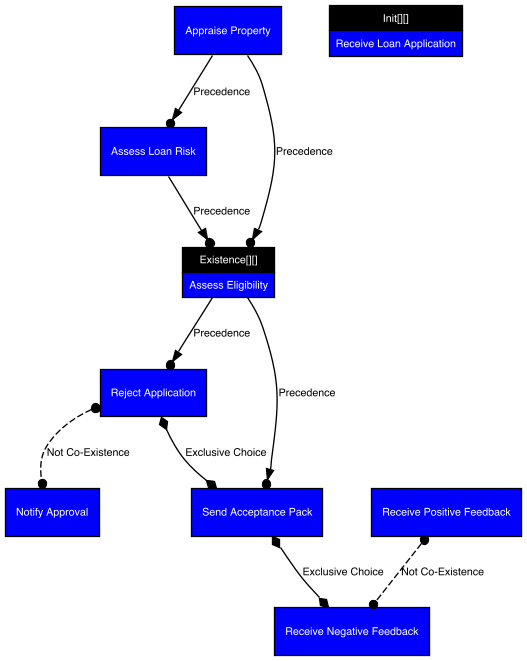
\includegraphics[width=0.6\columnwidth]{example1}
\caption{Loan approval declare process model }
\label{fig:ex}
\end{figure}

To test our approach, besides positive traces, we generated also negative traces. In particular, we generated traces that violate two different constraints:
% \todofc{Non ho messo il terzo test di violazione, perch\`e riguardava ancora una \emph{precedence}\ldots pensiamo se vogliamo aggiungerlo.}
\begin{enumerate}[label=(\textit{\alph*})]
\item the \emph{precedence(assess\_loan\_risk, assess\_eligibility)}, that is violated when either the latter activity is executed and the former is absent, or if both the activities appear in the log, but in the wrong temporal order;
%
\item the \emph{exclusive\_choice(send\_acceptance\_pack, receive\_negative\_feedback)}, that is violated when a trace either contains both the activities, or does not contain any of them.
\end{enumerate}
%
The resulting log consists of 64,000 positives traces, 25,600 traces that violate the constraint as in $(a)$, and 10,240 traces that violate the constraint as specified in $(b)$.
%
When fed with the positives traces and traces violating the constraint in $(a)$, our approach successfully manages to identify constraints that allow to clearly distinguish positives from negatives traces. Moreover, the discovered constraint coincides with the one we originally decided to violate during the generation phase. When confronted with the scenario $(b)$, our approach again successfully managed to identify a minimum model able to discriminate between positive and negative traces, and the identified constraint is indeed logically consistent with the constraint originally selected for the violation.
% In particular, it is worthy to notice that our approach derived 
Table \ref{tab:syntResults} summarize the obtained results and reports the first selected model for each scenario.

% source of this data:
% file:///Users/federico/Google%20Drive/on-negative-traces/experiments/2020-07-14%20Federico/run_experiments_2020-07-30_130357_CEST.html
\todoinfc{I tempi di calcolo riportati in tabella potrebbero non essere giusti. Chiedere a Sergio\ldots in particolare, Sergio suggeriva che per gli step \texttt{compatibles} e \texttt{choices} dovremmo prendere i tempi \texttt{user + system}; per lo step \texttt{opt} invece nel caso di minclose dovremmo prendere la \texttt{CPUtime}, mentre per la subsetclose dovremmo prendere \texttt{CPUtime * (numconstraints bigger model) } }
\begin{table}
\tiny
\begin{tabular}{c c c c p{2.8cm} | p{3cm}}
\hline
Scenario & \#pos & \#neg & time & Originally violated constraint & First discovered model \\
\hline\hline
$(a)$ & 64,000 & 25,600 & \bf{Total: \fpeval{81.78 + 1.94 + 109.74 + 3.32 + 15.165}s} & \emph{precedence(assess\_loan\_risk, assess\_eligibility)} & \emph{precedence(assess\_loan\_risk, assess\_eligibility)}\\
& & & Compatibles:  \fpeval{81.78 + 1.94}s  & & \\
& & & Choices:  \fpeval{109.74 + 3.32}s  & & \\
& & & Optimisation: 15.165s & & \\
%
\hline
%
$(b)$ & 64,000 & 10,240 & \bf{Total: \fpeval{81.78 + 1.94 + 94.51 + 2.96 + 1.379}s} & \emph{exclusive\_choice( send\_acceptance\_pack, receive\_negative\_ feedback)} & \emph{coExistence(reject\_application, receive\_negative\_feedback)}\\
& & & Compatibles:  \fpeval{81.78 + 1.94}s  & & \\
& & & Choices:  \fpeval{94.51 + 2.96}s  & & \\
& & & Optimisation: 1.379s & & \\
\hline
\end{tabular}
\caption{Models discovered when dealing with the synthetic data set.}
\label{tab:syntResults}
\end{table}

% PARAMETRI RuM usati:
% Templates: devi selezionarli tutti eccetto:
%  - not precedence
%  - not chain precedence
%  - not response
%  - not chain response
%  - not responded existence
% Constraint support: io ho provato 80,90 e 100 - qui penso che puoi vedere un po' in base ai risultati che ti escono
% Pruning types: come dicevo oggi li ho provati tutti e 4 ma secondo me e` sufficiente None.
% Vacuity detection: deve essere OFF
% Activity support filter: deve essere a 0%

For the sake of completeness, we decided to experiment also with the Process Discovery Tool of the Rum Framework\footnote{\url{https://rulemining.org/}}, that is based on the Declare Miner algorithm \cite{2018a-Maggi}. Based on the exploitation of positive traces only, Declare Miner discovers a rich model that describes as ``most exactly'' as possible the given traces. When fed with the positive traces of our artificial log, and with the \emph{coverage} parameter set to 100\% (i.e., prefer constraints that are valid for all the traces in the logs), the RuM Framework discovers a model made of 514 constraints. If the coverage is relaxed to 80\% (prefer constraints that are satisfied by at least the 80\% of the traces), the model cardinality grows up to 1031 constraints.

In both cases the discovered model is able to distinguish between the positive and the negative traces. This is not surprising, since Declare Miner aims to identify all the constraints that hold for a given log: hence, it will discover also those constraints that allow to discern positive from negative traces. Rather, this result is a clear indication that indeed our artificial log has been constructed ``correctly'', since negative traces differ from the positive ones for some specific constraints, and the positive traces exhaustively elicit the cases that can occur. 
%In a sense we could say that the log is sufficiently exhaustive of all positive cases that can occurr.Declare Miner performance are enhanced 
This is typical of artificial logs, while real-life logs might not enjoy these properties.
%
Another consideration is about the cardinality of the discovered model: the Declare Miner approach provides a far richer description of the positive traces, at the cost perhaps of bigger models. Our approach instead has the goal of identifying the \emph{smallest} set of constraints that allow to discriminate between positive and negatives. In this sense, approaches like the one presented in this paper and Declare Miner are complementary.

% \todoinfc{ChiaraDFM, qui ci starebbe bene un paragrafetto in cui riportiamo i risultati ottenuti usando RuM. Il commento che potremmo scrivere e' che RuM trova un modello intero per coprire le positive, e riesce a distingure benissimo anche le negative: il risultato e' atteso, dato l'elevato numero di tracce che rende il synthetic data set molto informativo.}






\subsection{Evaluation on case studies from real data}
\label{sec:realdata}

\todoindl{Chiara DFM\&Sergio\&Fabrizio: descrizione dataset e risultati di esperimenti coi dati veri}

For the experimentation with real datasets, we used three real-life event logs: \textsc{cerv}, \textsc{sepsis} and \textsc{bpic12}. Starting from these event logs we generated 5 different datasets, each composed of a set of positive and a set of negative traces, by applying different criteria to distinguish between positive and negative traces, i.e., by labeling the event log with different labeling functions. 

\textsc{cerv} is an event log related to the process of cervical cancer screening carried out in an Italian cervical cancer screening center~\cite{2007b-Lamma}. Cervical cancer is a disease in which malignant (cancer) cells form in the tissues of the cervix of the uterus. The screening program proposes several tests in order to early detect and treat cervical cancer. It is usually composed by five phases: Screening planning; Invitation management; First level test with pap-test; Second level test with colposcopy, and eventually biopsy. The traces contained in the event log have been analyzed by a domain expert and labeled as compliant (positive traces) or non-compliant (negative traces) with respect to the cervical cancer screening protocol adopted by the screening center.

\textsc{sepsis}~\cite{Sepsis} is an event log that records trajectories of patients with symptoms of the life-threatening sepsis condition in a Dutch hospital.
%Œ\textsc{Sepsis} is an event log that records trajectories of patients with symptoms of the life-threatening sepsis condition in a Dutch hospital. 
Each case logs events since the patient’s registration in the emergency room until her discharge from the hospital. Among others, laboratory tests together with their results are recorded as events. The traces contained in the event log have been labelled based on their cycle execution time. In the \textsc{sepsis$_{mean}$} dataset, traces with a cycle time lower than the mean duration of the traces in the event log ($\sim$ 28 days) have been labelled as positive, as negative otherwise. Similarly, in the \textsc{sepsis$_{median}$}, traces with a cycle time lower than the median duration of the traces in the event log ($\sim$ 5 days)  have been labeled as positive, as negative otherwise.  

\textsc{bpic12}~\cite{BPIC2012} is a real-life event log pertaining to the application process for personal loans or overdrafts in a Dutch financial institute. It merges three intertwined sub-processes. Also in this case, the traces have been labelled based on their cycle execution time. In the \textsc{bpic12$_{mean}$} dataset (resp. \textsc{bpic12$_{mean}$}), traces with a cycle time lower than the mean (resp. median) duration of the traces in the event log ($\sim$ 8 days, resp. $\sim$ 19 hours) have been labelled as positive, as negative otherwise. 

%The \textsc{cerv} event log has been labeled based on the compliance of th


Table~\ref{tab:rl_datasets} summarizes the data related to the five resulting datasets.

\begin{table} [h]
	\centering
	\scalebox{0.8}{
		\begin{tabular} {l l c c c c c}
		\toprule
			\multirow{2}{*}{\textbf{Dataset}} & \multirow{2}{*}{\textbf{Log}} & \multirow{2}{*}{\textbf{Trace \#}} & \multirow{2}{*}{\textbf{Activity \#}} & \multirow{2}{*}{\textbf{Label}} & \textbf{Positive} & \textbf{Negative}  \\ 
			& & & & & \textbf{Trace \#} & \textbf{Trace \#} \\ \midrule
			\textsc{cerv$_{compl}$} & \textsc{cerv} & 157 & 16 & compliant & 55 & 102 \\ \midrule
			\textsc{sepsis$_{mean}$} & \multirow{2}{*}{\textsc{sepsis}} & \multirow{2}{*}{1000} & \multirow{2}{*}{16} & mean duration & 838 & 212 \\
			\textsc{sepsis$_{median}$} &  &  &  & median duration & 525 & 525 \\ \midrule
			\textsc{bpic12$_{mean}$} & \multirow{2}{*}{\textsc{bpic12}} & \multirow{2}{*}{13087} & \multirow{2}{*}{36} & mean duration & 8160 & 4927  \\
			\textsc{bpic12$_{median}$} &  &  &  & median duration & 6544  & 6543 \\ 			
			\bottomrule
		\end{tabular}}
		\caption{Dataset description}
		\label{tab:rl_datasets}
\end{table}

Table~\ref{tab:rl_results} summarizes the results obtained by applying the \nd algorithm. In detail, the table reports for each dataset, (i) the results related to \minclos and \subsetclos - in terms of number of returned models\footnote{We stop generating models after $20$ models, i.e., \para{max} in Table~\ref{tab:rl_results} indicates that more than $20$ models have been returned.}, in terms of minimum size of returned models, as well as in terms of average percentage of negative traces excluded by the returned model. Moreover, the table reports the time required for computing the set of compatibles, the set of choices, as well as for \minclos and \subsetclos.

\begin{table} [h]
	\centering
	\scalebox{0.58}{
		\begin{tabular} {l | c c c | c c c | c c c c}
		\toprule
			\multirow{4}{*}{\textbf{Dataset}} & \multicolumn{3}{c|}{\textbf{\minclos}} & \multicolumn{3}{c|}{\textbf{\subsetclos}} & 	\multicolumn{4}{c}{\textbf{ Required Time (s)}} \\ \cmidrule{2-11}
			& \textbf{Number} & \textbf{Min} & \textbf{Avg.} & \textbf{Number} & \textbf{Min} & \textbf{Avg.} & \multirow{3}{*}{\textbf{Comp.}} & \multirow{3}{*}{\textbf{Choices}} & \multirow{3}{*}{\textbf{\minclos}} & \multirow{3}{*}{\textbf{\subsetclos}} \\			
			& \textbf{of} & \textbf{model} & \textbf{Violated} & \textbf{of} & \textbf{model} & \textbf{Violated} & & & & \\
			& \textbf{models} & \textbf{size} & \textbf{L$^{-}$ \%} & \textbf{models} & \textbf{size} & \textbf{L$^{-}$ \%} & & & & \\\midrule
			\textsc{cerv$_{compl}$} & \para{max} & 4 & 100\% & \para{max} & 4 & 100\% & 0.12 & 0.33 & 0.045 & 0.065 \\ \midrule
			\textsc{sepsis$_{mean}$} & 1 & 8 & 4.25\% & 1 & 8  & 4.25\% & 0.73 & 1.04 & 0.035 & 0.039 \\ 
			\textsc{sepsis$_{median}$} & 16 & 14 & 26.86\% & \para{max} & 14 & 26.86\% & 0.45 &	1.5 & 0.087 & 0.2 \\ \midrule
			\textsc{bpic12$_{mean}$} & \para{max} & 12 & 1.42\% & \para{max} & 12 & 1.42\% & 13.51 & 31 & 0.066 & 0.096  \\ 
			\textsc{bpic12$_{median}$} & \para{max} & 22 & 36.59\% & \para{max} & 23 & 36.59\% & 13.32 & 37.63 & 43.846 & 359.164 \\ 			
			\bottomrule
		\end{tabular}}
		\caption{Real Life log results}
		\label{tab:rl_results}
\end{table}

The table shows that for the \textsc{cerv$_{compl}$} dataset, \nd is able to return models that satisfy the whole set of positive traces and violate the whole set of negative traces (the percentage of violated traces in $L^-$ is equal to 100\%) with a very low number of constraints (4). For the other datasets, the returned models are always able to satisfy all the traces in $L^+$, however not all the negative traces are violated by the returned models. In case of the datasets built by using the mean of the trace cycle time, the percentage of violated traces is relatively small ($4.25\%$ for \textsc{sepsis$_{mean}$} and $1.24\%$ for \textsc{bpic12$_{mean}$}), as the number of constraints of the returned models ($8$ for \textsc{sepsis$_{mean}$} and $12$ for \textsc{bpic12$_{mean}$}). Nevertheless, \nd is able to obtain reasonable results with the real life datasets built with the median of the trace cycle time. Indeed, it is able to return models able to accept all the traces in $L^+$ and to cover about $27\%$ (resp. $37\%$) of the traces in $L^-$ for \textsc{sepsis$_{median}$} (resp. \textsc{bpic12$_{median}$}). The difference in terms of results between the  \textsc{cerv$_{compl}$} and the other datasets is not surprising. Indeed, while what characterizes positive and negative traces in the \textsc{cerv$_{compl}$} dataset depend upon the control flow (i.e., it depends on whether each execution complies with the cervical cancer screening protocol adopted by the screening center), when mean and median cycle time are used, the difference between positive and negative traces could likely not exclusively depend on the control flow of the considered traces. \todocdf{I would add the language bias in the discussion.}
The table also shows that \nd is overall very fast for small datasets (e.g., less than one minute for \textsc{cerv$_{compl}$}), while it requires some more time for large ones (e.g., \textsc{bpic12$_{mean}$} and \textsc{bpic12$_{median}$}). While the time required for computing \textit{compatibles} and \textit{choices} seems to be related to the size of the dataset, the time required for computing the closures seems to depend also on other characteristics of the datasets). 

We compared the obtained results with the ones obtained with state-of-the-art techniques for the discovery of declarative models starting (i) from  only positive traces; and (ii) from both positive and negative traces. 

%For the former case, we used the state-of-the-art Declare miner algorithm~\cite{2018a-Maggi}  implemented in the RuM toolkit~\cite{2020-Alman}. For the latter we compared the results obtained with \nd with the ones of DecMiner, the approach based on Inductive Logic Programming proposed in~\cite{2007b-Lamma}.

Concerning the classical declarative discovery from only positive execution traces, we used the state-of-the-art \declare miner algorithm~\cite{2018a-Maggi} implemented in the \rum toolkit~\cite{2020-Alman}. We used the \declareminer algorithm\footnote{We run the \declareminer algorithm with vacuity detection disabled, \par{activity support filter} set to 0\%, using both transitive closure and hierarchy-based reduction of the discovered constraints, as well as with all the Declare templates, except for \dec{NotResponse}, \dec{NotPrecedence}, \dec{NotChainPrecedence}, \dec{NotChainResponse}, \dec{NotRespondedExistence}.} to discover the \declare model starting from the only positive traces with different values of the \para{support} parameter, which measures the percentage of (positive) traces satisfied by the \declare model.  \todocdf{Move this part when the results are presented for the synthetic data}

Table~\ref{tab:rl_declare_miner} summarizes the obtained results. In detail, the table reports for each dataset and \para{support}, i.e., percentage of positive traces satisfied by the model, the size of the model in terms of number of constraints, as well as the percentage of negative traces violated by the model.

\begin{table} [h]
	\centering
	\scalebox{0.8}{
		\begin{tabular} {l l c c}
		\toprule
			\textbf{Dataset} & \textbf{\para{support}} & \textbf{Model size} & \textbf{Avg. violated L$^{-}$ \%}  \\ \midrule
			\multirow{2}{*}{\textsc{cerv$_{compl}$}} & 100\% & 323 & 9.8\% \\ 
			& 90\% & 517 & 100\% \\ \midrule
			\multirow{3}{*}{\textsc{sepsis$_{mean}$}} & 100\% & 210 & 4.25\%\\
			& 95\% & 342 & 81.13\% \\
			& 90\% & 363 & 100\% \\ \midrule
			\multirow{3}{*}{\textsc{sepsis$_{median}$}} & 100\% & 202 & 22.29\% \\ 
			& 95\% & 211 & 88.19\% \\
			& 90\% & 322 & 100\% \\ \midrule
			\multirow{3}{*}{\textsc{bpic12$_{mean}$}} & 100\% & 514 & 0\% \\
			& 90\% & 637 & 83.52\%\\ 
			& 80\% & 650 & 100\%\\ \midrule
			\multirow{3}{*}{\textsc{bpic12$_{median}$}} & 100\% & 532 & 14.21\% \\ 
			& 80\% & 654 & 98.18\% \\			
			& 60\% & 654 & 98.18\% \\	
		\bottomrule
		\end{tabular}}
		\caption{\declareminer results}
		\label{tab:rl_declare_miner}
\end{table}

Finally, we compared the results obtained with \nd with the ones of \decminer, the state-of-the-art approach using both positive and negative execution traces based on Inductive Logic Programming proposed in~\cite{2007b-Lamma}. To this aim, we run the same procedure described in~\cite{2007b-Lamma} on the same dataset (the \textsc{cerv$_{compl}$} dataset) used in the same paper. Five fold-cross validation was used, i.e., the \textsc{cerv$_{compl}$} dataset was divided into 5 sets and in each experiment 4 were used for training and the remaining one for testing. The average accuracy of the five executions is collected, where the accuracy is defined as the sum of the number of compliant traces that are correctly classified as compliant by the learned model and the number of non-compliant traces that are correctly classified as non-compliant by the learned model divided by the total number of traces. Table~\ref{tab:acc_results} reports the obtained accuracy values for the \decminer, the \declareminer (with different values of the \para{support} parameter) and the \nd (both for the \minclos and \subsetclos closure) approach.

\begin{table} [h]
	\centering
	\scalebox{0.8}{
		\begin{tabular} {l c c}
			\toprule
			 \decminer &  & 97.44\%\\ \midrule
			\multirow{3}{*}{\declareminer} & \para{support}=100\% & 48.53\%\\
			& \para{support}=90\% & 95.5\% \\
			& \para{support}=80\% & 96.15\% \\ 
			& \para{support}=10\% & 81.94\% \\ \midrule
			 \multirow{2}{*}{\nd} & \minclos & 97.57\% \\ 
        & \subsetclos & 97.38\% \\ 			
			\bottomrule
		\end{tabular}}
		\caption{Accuracy results obtained with \declareminer, \decminer and \nd}
		\label{tab:acc_results}
\end{table}





% !TEX root = ../deviant-tkde.tex

\section{Related work}
\label{sec:related}

Process discovery is generally considered a challenging task of process mining \cite{2012-Maggi}. The majority of works in this field are focused on discovering a process model from a set of input traces that are supposed compliant with it. In this sense, process discovery can be seen as the application of a machine learning technique to extract a grammar from a set of positive sample data. Angluin et al. \cite{1983-Angliun} provide an interesting overview on this wide field.
Differently from grammar learning, where the model is often expressed with automata, regular expressions or production rules, process discovery usually adopts formalisms that can express concurrency and synchronization in a more understandable way \cite{2009-Goedertier}. 
The language to express the model is a crucial point, which inevitably influences the learning task itself. Indeed, the two macro-categories of business process discovery approaches---procedural and declarative---differ precisely by the type of language to express the model. 
%: procedural approaches envisage to uncover structured processes, whereas declarative ones are more suitable for unstructured models. 
Well known examples of procedural process discoverers are the ones presented in the works \cite{2003-Weijters,2004-Aalst,2007-Gunther,2010-Aalst,2013-Leemans,2015-Guo,2017-Augusto}.
\tcolor{blue}{See  \cite{2019-Augusto,YUREK:2018ww} for systematic literature reviews of this field. }%In particular, the $\alpha$-algorithm \cite{2004-Aalst} is one of the first and most famous process discovery approaches. Its simple structure does not allow the discovery of complicated routing constructs and can be negatively influenced by the presence of noise in the log. Definitely more robust techniques are the heuristics miner \cite{2003-Weijters} and the fuzzy miner \cite{2007-Gunther}, which can deal with unbalanced, incomplete, or noisy logs. %The work \cite{2010-Aalst} seeks a overfitting/underfitting balance between different parts of the extracted model by means of a two-step approach. The first step builds a transition system from the observation of occurrence, sequence and multi-set of activities in the log's traces. The second step converts the transition system into a Petri net, which can easily express the procedural nature of the business process.
%In \cite{2019-Augusto}, Augusto et al. present an extensive review of the procedural approaches to process discovery with a BPMN or Petri net output. Similarly to our approach, the comparison between the various tools is conducted on the basis of fitness, precision, generalisation and complexity. %The result of this comparison highlights how Inductive Miner \cite{2015-Guo}, Evolutionary Tree Miner \cite{2013-Leemans}, and Split Miner \cite{2017-Augusto} outperform all the other approaches, despite being rather limited when dealing with large-scale unfiltered logs.
Like most procedural approaches, all these works contemplate the presence of non-informative noise in the log, which should be separated from the rest of the log and disregarded.
%Like most procedural approaches to process discovery, all the works described so far consider deviant examples as a form of non-informative noise in the log, which should be separated from the rest of the log and disregarded.
 
Traditional declarative approaches to process discovery stem from the necessity of a more friendly language to express loosely-structured processes. Indeed---as also pointed out by \cite{2012-Maggi}---process models are sometimes less structured than one could expect, so procedural discovery could produce spaghetti-models. In that case, a declarative approach is more suitable to briefly list all the required or prohibited behaviours in a business process.
Similarly to our technique, the one exposed by Maggi et al. in \cite{2011-Maggi} starts by considering the set of all activities in the log and building a set of all possible candidate Declare constraints. 
%
%Then, differently from our algorithm, the candidate Declare constraints are translated into the equivalent \ac{LTL} and checked (one at a time) against all the log content employing the technique of \cite{2005-Aalst}. The process continue until certain levels of recall and specificity are reached. 
The performance of this technique is improved in \cite{2012-Maggi}, 
% with an interesting two-step approach to both reduce the search space of candidate constraints and exclude from the model those \ac{LTL} formulas that are vacuously satisfied.
%Also the the work \cite{2012-Schunselaar} by Schunselaar et al. proposes a model refinement to efficiently exclude vacuously satisfied constraints. 
while \cite{2012-Schunselaar} proposes a model refinement to efficiently exclude vacuously satisfied constraints. 


The MINERFul approach described in \cite{2015-DiCiccio} proposes to employ four metrics to guide the declarative discovery approach: support, confidence and interest factor for each constraint w.r.t. the log, and the possibility to include in the search space constraints on prohibited behaviours.
Particularly relevant for our purposes is the work by Di Ciccio et al. \cite{2017-DiCiccio}, who focus on refining Declare models to remove the frequent redundancies and inconsistencies. The algorithms and the hierarchy of constraints described in that work were particularly inspiring to define our discovery procedure.
Similarly to the procedural approaches, all the declarative ones described so far do not deal with negative examples, although the vast majority of them envisage the possibility to discard a portion of the log by setting thresholds on the value of specific metrics that the discovered model should satisfy.
In the work \cite{2021-Back}  the authors propose a declarative miner for learning Dynamic Condition Response (DCR) graphs from event logs. Similarly to our approach, they focus on control-flow-related aspects only, and disregard timing, data and resource perspectives. Negative examples are not exploited in the learning process, but taken into account when measuring underfitting and overfitting of the resulting model.

%In the work ... the authors propose a declarative miner for learning Dynamic Condition Response (DCR) Graphs from event logs. Similarly to our approach, they focus only control-flow-related aspects disregarding timing, data and resource perspectives. Furthermore, their approach relays also on negative examples, albeit only in the evaluation step to measure underfitting and overfitting of the resulting model.

In the wider field of grammar learning, the foundational work by Gold \cite{1967-Gold} showed how negative examples are crucial to distinguish the right hypothesis among an infinite number of grammars that fit the positive examples. Both positive and negative examples are required to discover a grammar with perfect accuracy. Since process discovery does not usually seek perfection, but only a good performance according to defined metrics, it is not surprising that many procedural and declarative discoverers disregard the negative examples. Nonetheless, in this work we instead claim that negative traces are extremely important when learning declarative process models.%\tododl{qui ho levato alcuni lavori tradizionali su grammar learning.}
%Among traditional grammar learning approaches, the ones by Angluin \cite{1987-Angluin} and Mooney \cite{1995-Mooney} are particularly relevant for our work.
%The article \cite{1987-Angluin} focuses on identifying an unknown model referred as ``regular set'' and represented through Deterministic Finite-state Acceptor (DFA). Coherently with Gold's theory  \cite{1967-Gold}, Angluin propose a learning algorithm that starts from input examples of the regular set's members and non-members. The learning process is realised through the construction of an ``observation table''. The approach of Mooney et al. \cite{1995-Mooney} shows three different algorithms to learn Conjunctive Normal Form (CNF), Disjunctive Normal Form (DNF) and Decision trees from a set of positive and negative examples. 
 
The information contained in the negative examples is actively used in a subset of the declarative process discovery approaches \cite{2007-Lamma,2009-Chesani,2010-Bellodi,2016-Bellodi,slaats_weighing_2021}. All these works can be connected to the basic principles of the \ac{ICL} algorithm \cite{1995-DaRaedt}, whose functioning principle is intrinsically related to the availability of both negative and positive examples. 
The \ac{DPML} described in \cite{2007-Lamma, 2007b-Lamma} by Lamma et al. focuses on learning integrity constraints expressed as logical formulas. The constraints are later translated into an equivalent construct of the declarative graphical language DecSerFlow \cite{2006-Aalst}. Similarly to this approach, the DecMiner tool described in \cite{2009-Chesani}, learns a set of \tcolor{blue}{Social Constrained if-and-only-if (SCIFF) rules} \cite{2008-Alberti} which correctly classify an input set of labelled examples. Such rules are then translated into ConDec constraints \cite{2006-Pesic}. Differently from \cite{2009-Chesani}, the present work directly learns Declare constraints without any intermediate language.
%\tcolor{blue}{An important difference w.r.t our approach is precisely in the fact that \cite{2009-Chesani} expressly requires negative examples to perform the classification, whereas the algorithm we propose can work even in absence of counterexamples.\tododl{NO, 10 passa da rappresentazione SCIFF mentre noi lavoriamo direttamente sui template declare}}
\ac{DPML} has been later used in \cite{2010-Bellodi} to extract integrity constraints, then converted into Markov Logic formulas. %The weight of each formula is determined with a statistical relational learning tool. %Indeed, some process discovery approaches take inspiration from the methods to learn the probability distributions of stochastic generative grammars over sets of observed examples (1997,Ghahramani) (Kersting et al., 2006) (1997,Smyth) (2003,Cadez )
Taking advantage of the negative examples, the approach of \cite{2010-Bellodi}  is improved in \cite{2016-Bellodi}. %, thus obtaining significantly better results than other process discovery techniques. 
%
\tcolor{blue}{Another recent related work is the Rejection Miner by Slaats et al. \cite{slaats_weighing_2021}, which---analogously to our vision---considers process discovery as a binary classification task and provides an algorithm where some parts can be customised to include more constraints and different model minimisation strategies. Likewise, our approach envisages the possibility to employ a different language bias or closure operator.
%
Since the aim of \cite{slaats_weighing_2021} is to provide a general miner (not limited to Declare notation), they do not focus on  notation-specific improvements like our use of the closure to avoid redundancies and provide more compact models. 
%
%Notably, the authors of \cite{slaats_weighing_2021} report a set of real-life logs containing negative examples, which we employ in our evaluation. 
Interestingly, \cite{slaats_weighing_2021} also reports a demonstration of the reasons why Declare is not able to perfectly separate any pair of positive/negative traces. Consistently with this finding, our approach aims at discovering a model that accepts all traces in $L+$ and rejects as many traces in $L^-$ as possible. Despite its limits, we believe that Declare's diffusion in both industry and academia motivates the need to further investigate process discovery with this language.}

Since for all these works the availability of negative examples is crucial, recent years have seen the development of synthetical log generators able to produce not only positive but also negative process cases \cite{2019-Chesani,2017-Chesani,2020-Loreti,2009-Goedertier, 2014-Stocker, 2010-Hee}. In the experimental evaluation of this work, we employ the abductive-logic generator by Loreti et al. \cite{2020-Loreti} to synthesise part of the input event logs.
 
\tcolor{blue}{
Two-class declarative process discovery is sometimes related to sequence mining and classification \cite{2016-Fowkes,2017-Egho,2000-Zaki,2014-Lam,2020-DeSmedt}. In \cite{2016-Fowkes} the authors propose a probabilistic machine learning approach that infers subsequences which best compress a sequence database. 
A similar Bayesian technique is used by Egho et al.\cite{2017-Egho} to mine Standard Classification Rule Models, where the antecedent is the relevant subsequence, and the consequent expresses the support of that subsequence in each class.
%
The above-mentioned work by Maggi et al.\cite{2011-Maggi} originated from the idea that Apriori-like approaches %---such as sequence mining \cite{1994-Agrawal} and episode mining \cite{1997-Mannila}---
can discover local patterns in a log, but not rules representing prohibited behaviours and choices. 
The same motivation is behind the work by De Smedt et al. \cite{2020-DeSmedt}, which significantly enriches the expressiveness of the discovered models employing Declare behavioural constraints in sequence classification.
%Differently from \cite{2020-DeSmedt}, our work does not focus on characterising the traces of multiple input classes, but rather on the traditional process discovery tasks---where (at most) two disjoints classes of log traces are envisaged---and propose to extract from one class (the negative example set) the information relevant to characterise the other class (positive). In other words, the information that is relevant for our purpose is the fact that a trace \emph{does not belong} to a certain class.
Differently from \cite{2020-DeSmedt}, our work does not focus on characterising the traces of multiple, possibly intersected, input classes, but rather on refining the relevant feature of the traces belonging to a single class (the positive). In order to do so, we assume two disjunct sets of examples and suggest extracting from one class (the negative) the information relevant to characterise the other (the positive). In other words, the information that is relevant for our purpose is the fact that a trace \emph{does not belong} to a certain class.
%
Another important difference regards the mining algorithm: while \cite{2020-DeSmedt} explicitly considers each relevant Declare constraint, we envisage the language bias, as well as the subsumption hierarchy as input and we exploit the power of a satisfiability-based solver to determine the best model in terms of generality or simplicity. 
}

Particularly related to our approach are the works by Neider et al. \cite{2018-Neider}, Camacho et al. \cite{2019-Camacho}, and Reiner \cite{2019-Riener} where a \tcolor{blue}{satisfiability-based }solver is employed to learn a simple set of LTL formulas consistent with an input data set of positive and negative examples. In particular, Neider et al. \cite{2018-Neider} employ decision tree to improve the performance and manage large example sets; Camacho et al. \cite{2019-Camacho} exploit the correspondence of LTL formulae with Alternating Finite Automata (AFA); whereas Reiner \cite{2019-Riener} uses partial Directed Acyclic Graphs (DAGs) to decompose the search space into smaller subproblems.
Furthermore, the concept of negative example used in this work could be related to both the definitions of syntactical and semantic noise of \cite{2009-Gunther}. %In particular, besides being able to extract relevant syntactic information that characterise the positive examples w.r.t. negative, our approach could also be useful to deal with the semantic concept of modification noise i.e., the semantic difference between traces from the same process model, which has been partially or totally modified at a certain point in time.  
 
It is important to underline that also a limited number of procedural approaches envisage the need for taking into account the information contained into the negative examples. 
In particular, the work \cite{2015-Ponce} showed how negative examples can be employed to alleviate problems like log incompleteness and noise.
The \tcolor{blue}{Artificially Generated Negative Events (AGNEs) }tool described in \cite{2009-Goedertier} increases the dimension of an event log with artificially generated negative examples, then uses \ac{ILP} multi-relational classification to discover a Petri net model. 
Negative examples are generated in a rather syntactical way, by adding a unique negative event at the end of a positive trace. This concept is extended in the work of Ponce de Leon et al. \cite{2018-Ponce} which envisage the concatenations of a sequence of negative events. Differently from these approaches, our technique does not assume syntactical restrictions on the input negative examples.
%
\ac{ILP} is also used in \cite{2006-Ferreira}, where the authors suppose a set of negative examples provided by domain experts. The approach uses partial-order planning to discover a structured model. %More recently, the works \cite{2014-Broucke,2014-BrouckePhD} showed how synthetically generated traces can be employed to improve the robustness of the compliance monitor task. 
 
Deviant cases---intended as traces whose sequence of activities deviates from the expected behaviour---are the subject of deviance mining approaches reviewed and evaluated by Nguyen et al. in \cite{2016-Nguyen}. Some applications of deviance mining tend to highlight the differences between models discovered from deviant and non-deviant traces \cite{2014-Suriadi,2014-Armas}. Other works intend deviance mining as a classification task, where the miner is required to identify normal and deviant traces given a set of examples. The classification inherently causes the discovery of patterns which distinguish different types of traces. In this sense, deviance mining is particularly similar to sequence classification. The discovered patterns can be based on the simple frequency of individual activities as in \cite{2013-Suriadi,2015-Partington}, their co-occurrence as in \cite{2011-Swinnen}, or the occurrence of specific subsequences \cite{2013-Bose,2007-Lo,2016-Bernardi}.
Table \ref{tab:rw} briefly illustrate the classification of the cited related works.
\begin{table} [ht]
	\centering
	\renewcommand{\arraystretch}{1.5}
	%\scalebox{0.8}{
		\begin{tabular} {l | c |>{\centering\arraybackslash}m{.35\columnwidth}}
		\toprule
			\multirow{3}{*}{\textbf{Procedural} }& One-class discovery &\cite{2003-Weijters,2004-Aalst,2007-Gunther,2010-Aalst,2013-Leemans,2015-Guo,2017-Augusto,YUREK:2018ww} \\ \cline{2-3}		
				& Two-class discovery & \cite{2015-Ponce,2018-Ponce,2006-Ferreira} \\ \cline{2-3}	
				& Log generation & \cite{2009-Goedertier, 2014-Stocker,2010-Hee} \\ \midrule
			\multirow{3}{*}{\textbf{Declarative} }& One-class discovery &  \cite{2011-Maggi,2012-Maggi,2012-Schunselaar, 2015-DiCiccio, 2017-DiCiccio, 2021-Back} \\ \cline{2-3}						
				& Two-class discovery & \cite{2007-Lamma,2009-Chesani,2010-Bellodi,2016-Bellodi,slaats_weighing_2021,2007b-Lamma,2018-Neider,2019-Camacho,2019-Riener} \\ \cline{2-3}
				& Log generation & \cite{2019-Chesani,2017-Chesani,2020-Loreti} \\ \midrule
			\multicolumn{2}{l|}{\textbf{Deviance mining} } & \cite{2016-Nguyen,2014-Suriadi,2014-Armas,2013-Suriadi,2015-Partington,2013-Bose,2007-Lo,2016-Bernardi,2011-Swinnen} \\ \midrule
			\multicolumn{2}{l|}{\textbf{Sequence mining/classification} } & \cite{2016-Fowkes,2017-Egho,2000-Zaki,2014-Lam,2020-DeSmedt} \\ 
		\bottomrule
		\end{tabular}
		%}
		\caption{Classification of related works.}
		\label{tab:rw}
\end{table}
 
 
 
%Add someware something on Discovery with DCR graphs (https://dblp.uni-trier.de/pers/hd/s/Slaats:Tijs) https://link.springer.com/chapter/10.1007%2F978-3-030-21290-2_37
%
%https://link.springer.com/chapter/10.1007%2F978-3-642-32885-5_6
%http://ceur-ws.org/Vol-1021/paper_10.pdf
%
%negation of declare constraints:
%https://www.researchgate.net/publication/284570318_Patterns_for_a_Log-Based_Strengthening_of_Declarative_Compliance_Models
%
%process mining ibrido
%https://link.springer.com/article/10.1007/s13740-020-00112-9

%% !TEX root = ../deviant.tex

\section{Discussion}
\label{sec:discuss}\tododl{x Dani: sezione da raffinare alla fine. Molte riflessioni penso non abbiano pi\` u senso.}

It is worth to underline that a declarative process discoverer taking advantage of explicitly defined positive and negative examples is not necessarily an alternative to procedural discovery techniques. 
Indeed in some cases, when correct thresholds and language biases are adopted, procedural discoverers have the great advantage to provide the user with a rather easy-to-understand definition of the process model. Nonetheless, the informative content provided by those process cases that are discarded by procedural discoverer (e.g., in order to avoid spaghetti models) can still be extremely important. 
A declarative process discoverer taking advantage of explicitly defined positive and negative examples can extract valuable information from such discarded traces and synthesize it into declarative constraints. The resulting output would be an hybrid procedural/declarative process model, showing a simple and handy structured representation of the main business process together with a set of declarative constraints. The goal of such constraints would be to account for less frequent deviances and prohibited behaviours in a much more synthetic and easy-to-understand way with respect to an equivalent spaghetti-like procedural formulation.

Furthermore, such hybrid solution could also greatly simplifying the elicitation of long-term dependencies between activities that occur at the beginning of the process and those carried out towards the end. Indeed, the structured nature of procedural approaches makes them not properly suitable to express such dependencies.
One current way to tackle such issue is through the employment of global variables and if statements to control the execution flow of each instance.
Kalenkova et al. (2020, Kalenkova)  propose e process discovery technique devoted to repair free-choice procedural workflows with additional modeling constructs, which can more easily capture non-local dependencies. Nonetheless, since such additional constraints are intended to preserve the procedural nature of the model, the result may increase its complexity and ultimately affect its readability.
An hybrid procedural/declarative model formulation would maintain a structured form to express the model while integrating it with handy declarative long-term constraints involving activities occurring far from each other in the workflow.

For example, consider the load application process depicted in Fig. ... The procedural nature of the model makes it particularly easy to understand for a human subject. Nonetheless, if we want to add a rather simple constraint such as: "Do not ask customer feedback if the application was cancelled", a substantial modification of the model is required.
Indeed, the model must state that the branch including "Cancel application" (and then "Notify cancellation") must be followed by the END event, whereas any other branch can still include "Ask for customer feedback" before the END event.
In practice, adding a constraint of such kind force us to add a alternative branch towards the end of the model.
If many alternative paths are present in the model and we need to add many conditions of this kind, the diagram in Fig.. may quickly turn into a spaghetti model.


A more compact and readable way to apply this modification is to maintain the present process model structure and equipping it with a declarative elicitation of the prohibited behaviours. In the considered case, the simple inclusion of a constraint such as "NOT PRECEDENCE(Cancel application, Ask for customer feedback)" prevents all forbidden paths. 

This idea of a hybrid procedural/declarative model formulation has been explored by various works and proved to be particularly effective in the field of medical clinical guidelines (2009a, Bottrighi) (2009b, Bottrighi) (2011, Bottrighi). A wider landscape of applications is considered by Maggi et al. in the work (2018b, Maggi). The technique starts from a structured business process model and adopts non-deterministic finite-state automaton manipulation to detect violations of compliance requirements expressed as temporal declarative rules.

% !TEX root = ../deviant.tex

\section{Conclusion}
While the vast majority of works see process discovery as a one-class supervised learning task, we embrace the less popular view of process discovery as a binary supervised learning job, where traces that deviate from the expected behaviour can be considered as heralds of valuable information about the process itself. Devoted to this vision, we developed a technique which considers both positive and negative traces and performs process discovery as a satisfiability problem, where different heuristics can be adopted to assess the optimal model according to different goals.  
\todoindl{Io vedrei bene qui gli argomenti attualmente in Discussion narrati come future works... }
Finally, the performance of the technique presented in this paper could be boosted through a parallel approach. Analogously to previous works \cite{2018a-Maggi, 2018-Loreti, 2020b-Loreti} we can envisage two possible directions to decompose our task: by spitting the model (i.e. in this case the set of constraints to be learned), or the input data (i.e. the business log). The algorithm presented here could easily adopt the first kind of partitioning, whereas the second might be more challenging.




% use section* for acknowledgment
\ifCLASSOPTIONcompsoc
  % The Computer Society usually uses the plural form
  \section*{Acknowledgments}
\else
  % regular IEEE prefers the singular form
  \section*{Acknowledgment}
\fi

This work was partially supported by the European Commission funded projects ``Humane AI: Toward AI Systems That Augment and Empower Humans by Understanding Us, our Society and the World Around Us'' (grant \# 820437) and ``AI4EU: A European AI On Demand Platform and Ecosystem'' (grant \# 825619). The support is gratefully acknowledged.

%\section*{References}

\bibliographystyle{IEEEtran}

\bibliography{deviant}
% !TEX root = ../deviant.tex

\begin{acronym}[PUB/SUB]
    \acro{ASP}{Answer Set Programming}
    \acro{ILP}{Inductive Logic Programming}
\end{acronym}



\begin{IEEEbiography}[{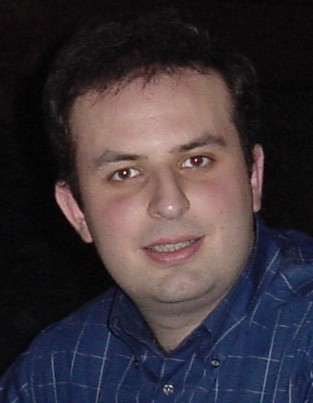
\includegraphics[width=1in,height=1.25in,clip,keepaspectratio]{img/Chesani.jpg}}]{Federico Chesani}, 
Ph.D. in Computer Science, is associate professor of Computer Science at DISI---University of Bologna. His research activities focus on the area of Logic Programming, Business Processes Modelling, Distributed Verification and Monitoring, and Rule-based Decision Support Systems.
\end{IEEEbiography}

\begin{IEEEbiography}[{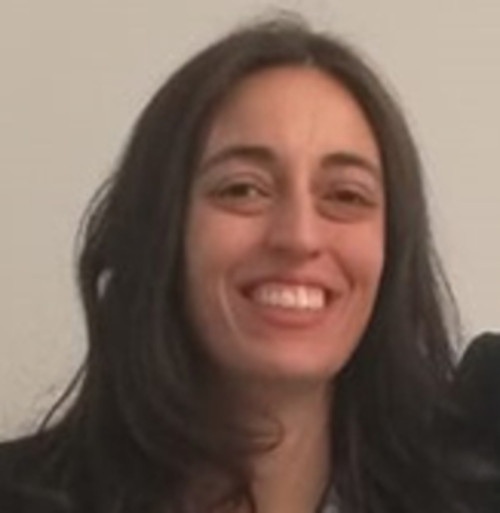
\includegraphics[width=1in,height=1.25in,clip,keepaspectratio]{img/Difrancescomarino.png}}]{Chiara Di Francescomarino}
is a researcher at Fondazione Bruno Kessler in the Process and Data Intelligence  Unit.  She received her PhD in Information and Communication Technologies from the University of Trento, working on business process modeling and reverse engineering from execution logs. She is currently working in the field of process mining, investigating problems related to process monitoring, process discovery, as well as predictive process monitoring. She has published papers in the top business process conferences and journals and she has worked in local and international research projects. 
\end{IEEEbiography}

\begin{IEEEbiography}[{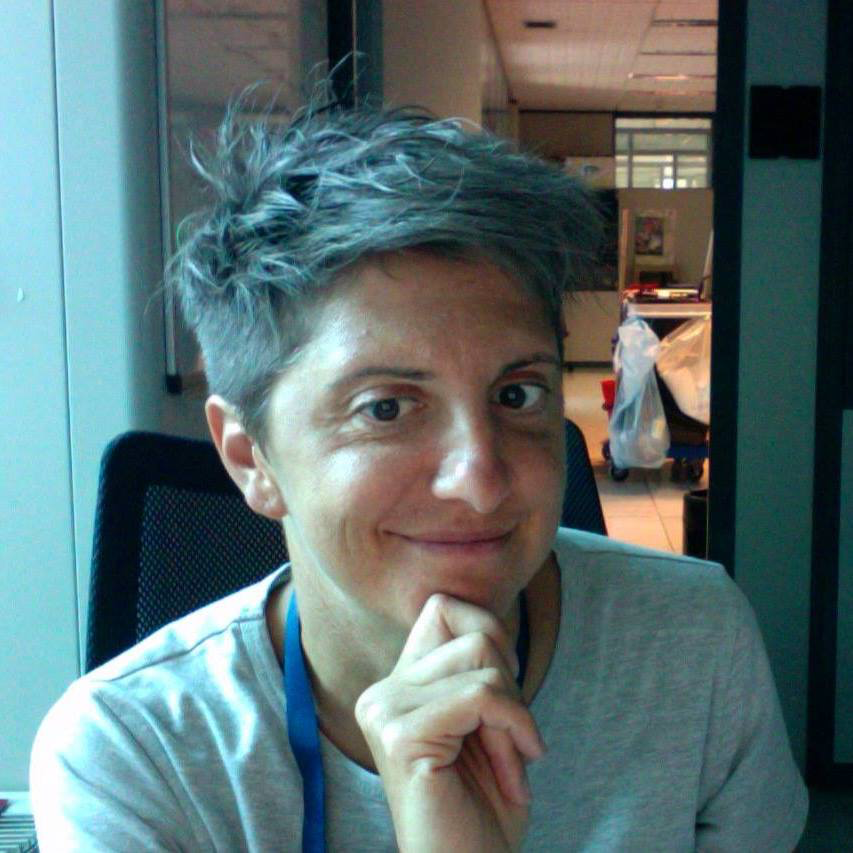
\includegraphics[width=1in,height=1.25in,clip,keepaspectratio]{img/Ghidini.png}}]{Chiara Ghidini}
is a Senior Research Scientist at Fondazione Bruno Kessler where she leads the Process \& Data Intelligence Research Unit.  
Her scientific work in the areas of Semantic Web, Knowledge Engineering and Representation, Multi-Agent Systems and Process Mining is internationally well known and recognised, and she has actively been involved in the organisation of several reference conferences in these areas. She is a board member of the Italian Association for Artificial Intelligence and is involved in the scientific coordination of the Centre for Digital Health and Well Being of Head of Fondazione Bruno Kessler.
\end{IEEEbiography}

\begin{IEEEbiography}[{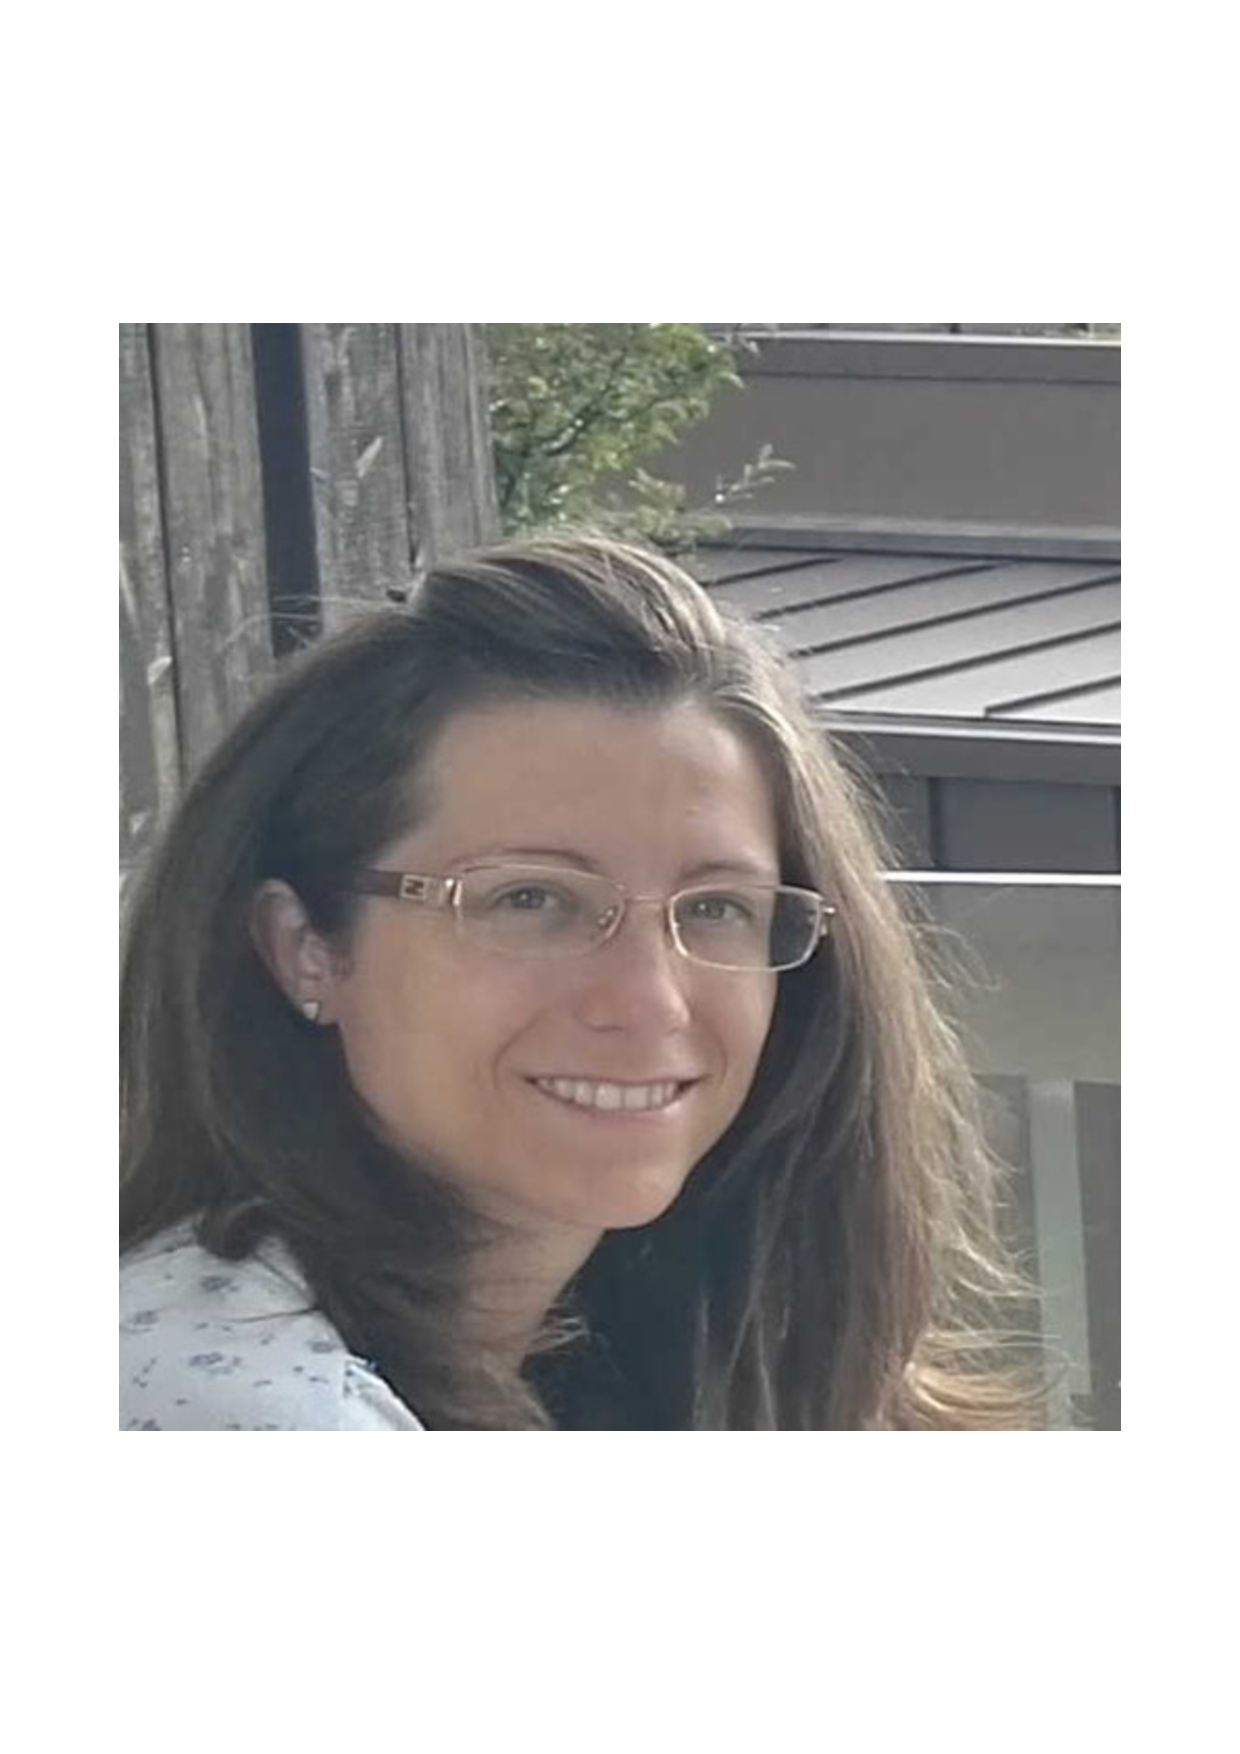
\includegraphics[width=1in,height=1.25in,clip,keepaspectratio]{img/Loreti.pdf}}]{Daniela Loreti}
is junior assistant professor of Operating Systems at Department of Computer Science and Engineering, University of Bologna. She received her Ph.D. in Computer Science in 2016. 
Her research focuses on distributed systems for big data management and stream processing as well as parallel paradigms for high performance computing. She is also interested in the parallelization of artificial intelligence techniques in the fields of machine learning, process mining and expert systems.
\end{IEEEbiography}

\begin{IEEEbiography}[{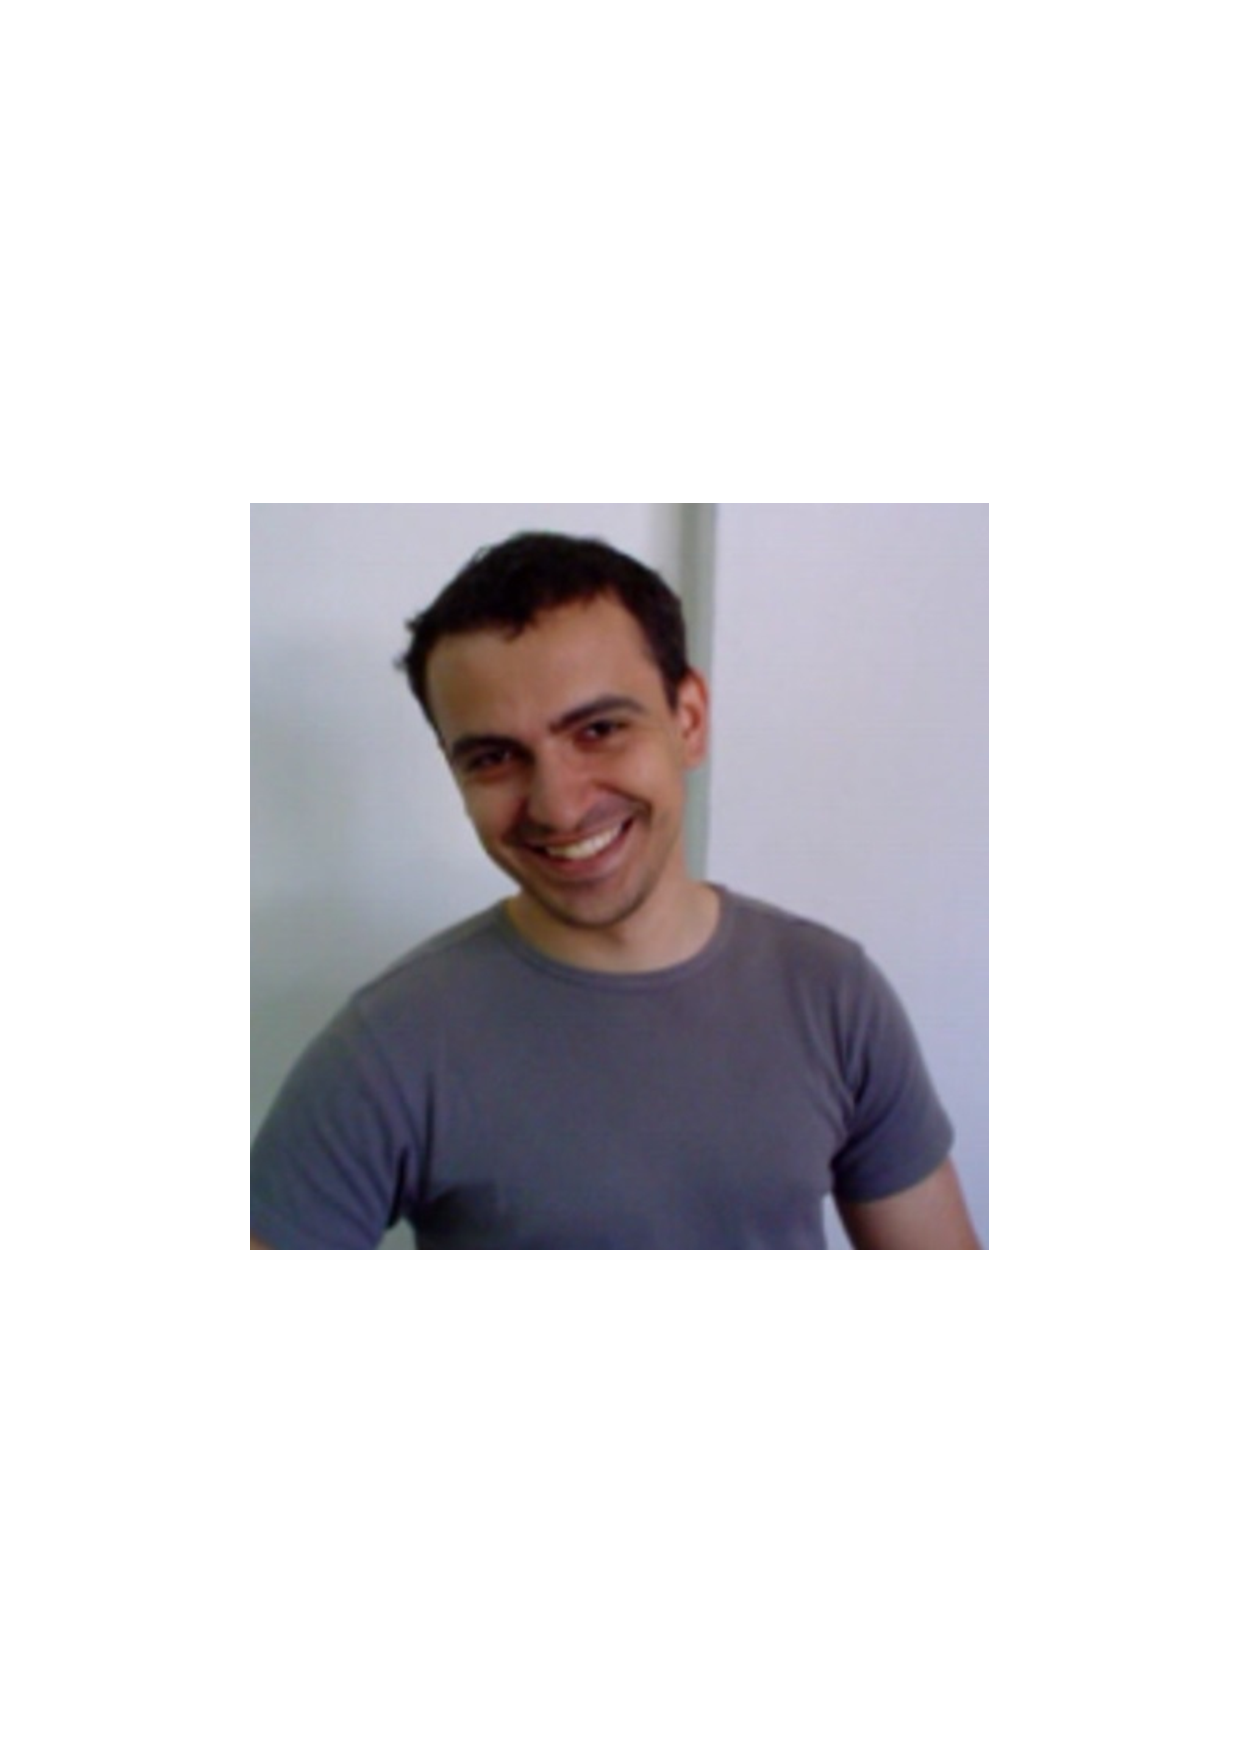
\includegraphics[width=1in,height=1.25in,clip,keepaspectratio]{img/Maggi.pdf}}]{Fabrizio Maria Maggi}
is Associate Professor at the KRDB Research Centre for Knowledge and Data. He devises techniques grounded in business process management, process mining, predictive analytics and his work is specifically focused on the application of artificial intelligence and machine learning in the context of business process analytics. On these topics, he authored more than 130 papers, appeared in top-tier, international journals and conferences. He is recipient of 4 best paper awards, two of which in the International Conference on Business Process Management. 
\end{IEEEbiography}

\begin{IEEEbiography}[{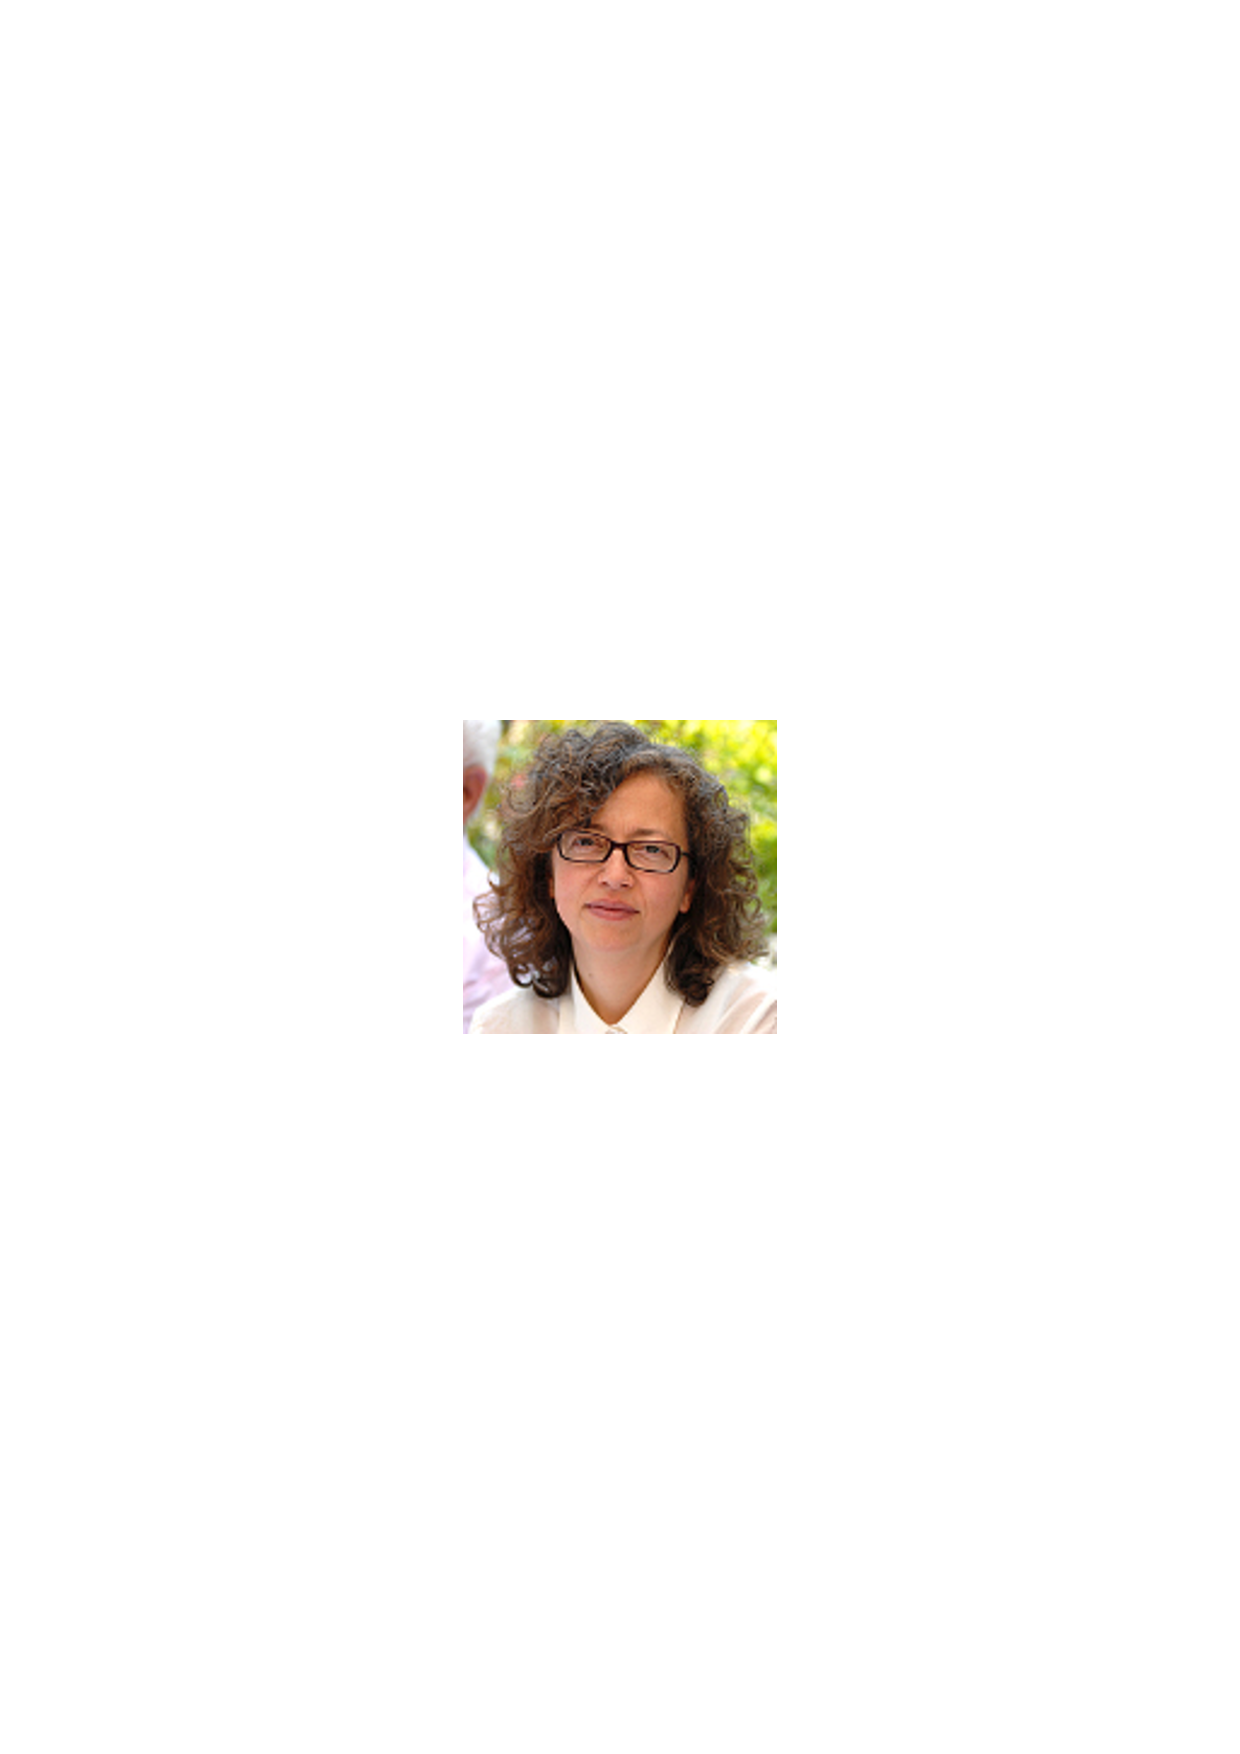
\includegraphics[width=1in,height=1.25in,clip,keepaspectratio]{img/Mello.pdf}}]{Paola Mello}
is Full Professor at the University of Bologna, where she conducts research, both practical and theoretical in Artificial Intelligence. In particular, her research activity is  about knowledge representation, computational logic, multi-agent and  decision support systems, with applications in medicine, web services, business processes, monitoring and verification.  She has been President of the Italian Association for Artificial Intelligence and Head of the Department of Computer Science and Engineering of the University of Bologna. She is fellow of the European Association for Artificial Intelligence.
\end{IEEEbiography}

\begin{IEEEbiography}[{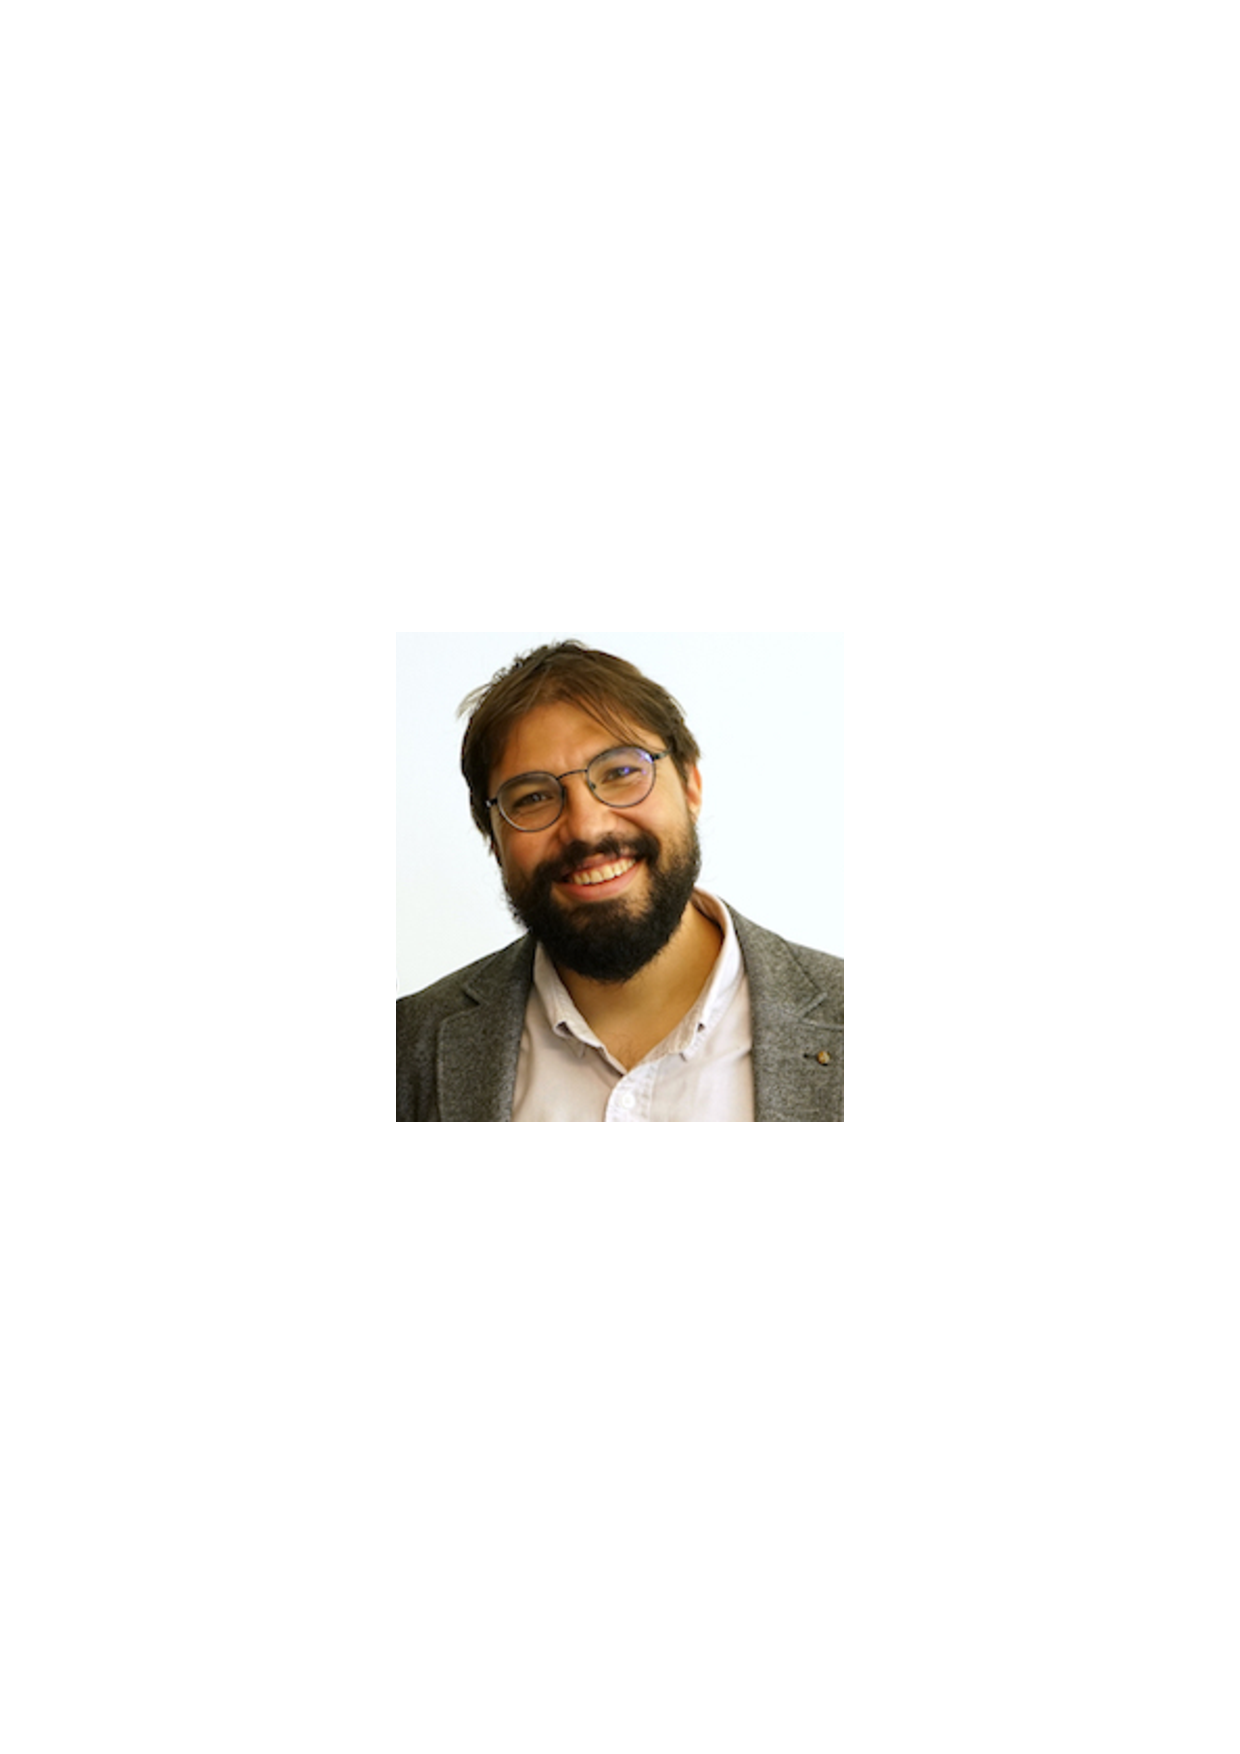
\includegraphics[width=1in,height=1.25in,clip,keepaspectratio]{img/Montali.pdf}}]{Marco Montali}
is Full Professor and Vice-Dean for Studies at the Faculty of Computer Science, Free University of Bozen-Bolzano, Italy, where he also coordinates the MSc Program in Computational Data Science. He investigates foundational and applied techniques grounded in artificial intelligence and formal methods for the model- and data-driven analysis of business processes and multiagent systems. He is member of the Steering Committee of the IEEE Task Force on Process Mining. He is co-author of more than 200 papers, many of which in top-tier conferences and journals, and recipient of 8 best paper awards.\end{IEEEbiography}


\begin{IEEEbiography}[{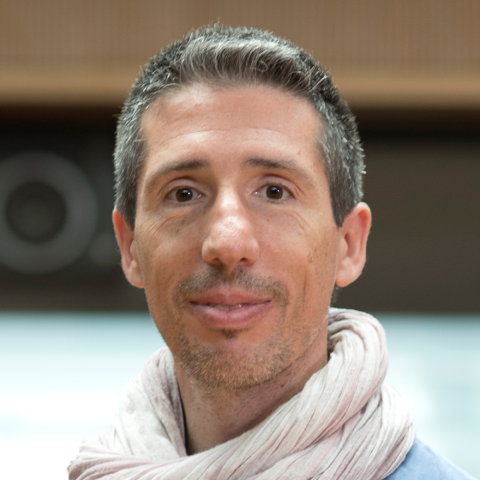
\includegraphics[width=1in,height=1.25in,clip,keepaspectratio]{img/Tessaris.png}}]{Sergio Tessaris}
received the PhD degree in computer science from the University of Manchester (UK). He is Assistant Professor at the Faculty of Computer Science of the Free University of Bozen-Bolzano (Italy). His research interests include the use of Semantic Technologies and Knowledge Representation formalisms to support the management, access, and exploitation of data and processes.
\end{IEEEbiography}

\vfill

\end{document}